% Options for packages loaded elsewhere
\PassOptionsToPackage{unicode}{hyperref}
\PassOptionsToPackage{hyphens}{url}
%
\documentclass[
]{book}
\usepackage{amsmath,amssymb}
\usepackage{lmodern}
\usepackage{ifxetex,ifluatex}
\ifnum 0\ifxetex 1\fi\ifluatex 1\fi=0 % if pdftex
  \usepackage[T1]{fontenc}
  \usepackage[utf8]{inputenc}
  \usepackage{textcomp} % provide euro and other symbols
\else % if luatex or xetex
  \usepackage{unicode-math}
  \defaultfontfeatures{Scale=MatchLowercase}
  \defaultfontfeatures[\rmfamily]{Ligatures=TeX,Scale=1}
\fi
% Use upquote if available, for straight quotes in verbatim environments
\IfFileExists{upquote.sty}{\usepackage{upquote}}{}
\IfFileExists{microtype.sty}{% use microtype if available
  \usepackage[]{microtype}
  \UseMicrotypeSet[protrusion]{basicmath} % disable protrusion for tt fonts
}{}
\makeatletter
\@ifundefined{KOMAClassName}{% if non-KOMA class
  \IfFileExists{parskip.sty}{%
    \usepackage{parskip}
  }{% else
    \setlength{\parindent}{0pt}
    \setlength{\parskip}{6pt plus 2pt minus 1pt}}
}{% if KOMA class
  \KOMAoptions{parskip=half}}
\makeatother
\usepackage{xcolor}
\IfFileExists{xurl.sty}{\usepackage{xurl}}{} % add URL line breaks if available
\IfFileExists{bookmark.sty}{\usepackage{bookmark}}{\usepackage{hyperref}}
\hypersetup{
  pdftitle={Economics},
  pdfauthor={Dyrehaugen Web Notebook},
  hidelinks,
  pdfcreator={LaTeX via pandoc}}
\urlstyle{same} % disable monospaced font for URLs
\usepackage{longtable,booktabs,array}
\usepackage{calc} % for calculating minipage widths
% Correct order of tables after \paragraph or \subparagraph
\usepackage{etoolbox}
\makeatletter
\patchcmd\longtable{\par}{\if@noskipsec\mbox{}\fi\par}{}{}
\makeatother
% Allow footnotes in longtable head/foot
\IfFileExists{footnotehyper.sty}{\usepackage{footnotehyper}}{\usepackage{footnote}}
\makesavenoteenv{longtable}
\usepackage{graphicx}
\makeatletter
\def\maxwidth{\ifdim\Gin@nat@width>\linewidth\linewidth\else\Gin@nat@width\fi}
\def\maxheight{\ifdim\Gin@nat@height>\textheight\textheight\else\Gin@nat@height\fi}
\makeatother
% Scale images if necessary, so that they will not overflow the page
% margins by default, and it is still possible to overwrite the defaults
% using explicit options in \includegraphics[width, height, ...]{}
\setkeys{Gin}{width=\maxwidth,height=\maxheight,keepaspectratio}
% Set default figure placement to htbp
\makeatletter
\def\fps@figure{htbp}
\makeatother
\setlength{\emergencystretch}{3em} % prevent overfull lines
\providecommand{\tightlist}{%
  \setlength{\itemsep}{0pt}\setlength{\parskip}{0pt}}
\setcounter{secnumdepth}{5}
\usepackage{booktabs}
\usepackage{amsthm}
\makeatletter
\def\thm@space@setup{%
  \thm@preskip=8pt plus 2pt minus 4pt
  \thm@postskip=\thm@preskip
}
\makeatother

\renewcommand\chaptername{}
\ifluatex
  \usepackage{selnolig}  % disable illegal ligatures
\fi
\usepackage[]{natbib}
\bibliographystyle{apalike}

\title{Economics}
\author{Dyrehaugen Web Notebook}
\date{2021-04-29}

\begin{document}
\maketitle

{
\setcounter{tocdepth}{1}
\tableofcontents
}
\hypertarget{economics}{%
\chapter{Economics}\label{economics}}


\includegraphics{fig/zelda.jpg}

The `science' of maximizing and minimizing stuff you can't measure.

The cult of math modl-ing.
\href{pdf/Thomas_Palley_2106_Life_among_the_Econ_50yrs.pdf}{Palley (2021) Life among the Econs - 50 years on (pdf)}

\hypertarget{scarcity}{%
\chapter{Scarcity}\label{scarcity}}

\textbf{There is no Scarcity}

When we look at the world in terms of real resources and energy (i.e., the stuff of provisioning), it becomes clear that there is no scarcity at all. The problem isn't that there's not enough, the problem, again, is that it is maldistributed. A huge chunk of global commodity production is totally irrelevant to human needs and well-being. Consider all the resources and energy that are mobilized for the sake of fast fashion, throwaway gadgets, single-use stadiums, SUVs, bottled water, cruise ships and the military-industrial complex. Consider the scale of needless consumption that is stimulated by manipulative advertising schemes, or enforced by planned obsolescence. Consider the quantity of private cars that people have been forced to buy because the fossil fuel industry and automobile manufactures have lobbied so aggressively against public transportation. Consider that the beef industry alone uses nearly 60\% of the world's agricultural land, to produce only 2\% of global calories.

There is no scarcity. Rather, the world's resources and energy are appropriated (disproportionately from the global South) in order to service the interests of capital and affluent consumers (disproportionately in the global North). We can state it more clearly: our economic system is not designed to meet human needs; it is designed to facilitate capital accumulation. And in order to do so, it imposes brutal scarcity on the majority of people, and cheapens human and nonhuman life. It is irrational to believe that simply ``growing'' such an economy, in aggregate, will somehow magically achieve the social outcomes we want.

\href{https://www.jasonhickel.org/blog/2021/2/21/is-the-world-poor-or-unjust}{Hickel}

\hypertarget{rationing}{%
\chapter{Rationing}\label{rationing}}

\emph{Climate Change Economics}

Curbing consumption can be done either through rationing or draconian taxation. Both are feasible technically although their political acceptability may not be the same.

If one were to use rationing, one could introduce physical targets: there will be only x liters of gas per car annually and no family will be allowed to have more than two cars; or y kilograms of meat per person per month; or z kilowatts of electricity per household per month (or rolling blackouts). Clearly, there may be a black market for gas or meat, but the overall limits will be observed simply because they are given by the total availability of coupons. Some people might think that rationing is extraordinary, and I agree with them. But it has been done in a number of countries under wartime, and at times even during peacetime conditions, and it has worked. If indeed we face an emergency of such ``terminal'' proportions as the advocates of climate change claim, I do not see any reason why we should not resort to extreme measures.

\href{http://glineq.blogspot.com/2021/02/climate-change-covid-and-global.html}{Milanovic}

\hypertarget{taxing}{%
\chapter{Taxing}\label{taxing}}

\emph{Climate Change Economics}

But another approach (draconian taxation) is possible too. Instead of limiting physical quantities of goods and services that fulfill criteria (a) and (b) we would impose extremely heavy taxes on them. There is always a tax rate that would drive consumption of a good down to the level that we have in mind. It is here that I think we can use---again if we believe that the climate emergency is so dire---the lessons of covid.

Economic dislocations would be huge. It is not only the question of the entire upper middle class and the rich in advanced countries (and, as we have seen, elsewhere) losing significant parts of their real income as prices of most ``staple'' commodities (for them) increase by two, three or ten times; the dislocation will affect large sectors of the economy.

The effects will trickle down: unemployment will increase, incomes will plummet, the West will record the largest real income decline since the Great Depression.

However if such policies were steadfastly pursued for a decade or two, not only would emissions plummet too (as they have done in 2020), but our behavior and ultimately the economy would adjust. People will find jobs in different activities that will remain untaxed and thus relatively cheaper and whose demand will go up. Revenues collected from taxing ``bad'' actvities may be used to subsidize ``good'' activities or retrain people who have lost their jobs.

This is not magical thinking. These are policies that, with intergovernmental cooperation, knowledge of economics, data on global inequality, and the experience of covid, could be implemented.

\href{http://glineq.blogspot.com/2021/02/climate-change-covid-and-global.html}{Milanovic}

\hypertarget{nudging}{%
\chapter{Nudging}\label{nudging}}

\hypertarget{randomness}{%
\section{Randomness}\label{randomness}}

\emph{Memo}

There is strong evidence from the lab that people have misperceptions about what randomness looks like. When a person is asked to generate a series that approximates the flipping of a coin, they will alternate between heads and tails too often, and balance the frequencies of heads and tails over too short a sequence. When people are asked to judge which of two different sequences of coin flips are more likely, they tend to pick sequences with more alternation, despite their probability being the same.

What happens we look for a failure to perceive randomness in the outside world? Out of the lab?

When people watch basketball, they often see a hot hand. They will describe players as ``hot'' and ``in form''. Their belief is that the person who has just hit a shot or a series of shots is more likely to hit their next one.

But is this belief in the ``hot hand'' a rational belief? Or is the hot hand an illusion, whereby, just like they do with coins, they are seeing streaks in what is actually randomness?

In a famous examination of this question, Thomas Gilovich, Robert Vallone and Amos Tversky took shot data from a variety of sources, including the Philadelphia 76ers and Boston Celtics, and examined it for evidence of a hot hand.

What did they find? The hot hand was an illusion. As Daniel Kahneman wrote in Thinking, Fast and Slow when describing this research:

\begin{quote}
The hot hand is entirely in the eye of the beholders, who are consistently too quick to perceive order and causality in randomness. The hot hand is a massive and widespread cognitive illusion.
\end{quote}

Possibly even more interesting was the reaction to the findings from those in the sporting world. Despite the analysis, many sports figures denied that it could be true. Red Auerbach, who coached the Boston Celtics to nine NBA championships, said ``Who is this guy? So he makes a study. I couldn't care less.''

This provides another insight, about which Gilovich wrote:

\begin{quote}
The story of our research on the hot hand is only partly about the misperception of random events. It is also about how tenaciously people cling to their beliefs even in the face of hostile evidence.
\end{quote}

So, this isn't just about the misperception of the hot hand, but also about the failure of people to see their error when presented with evidence about it.

Let's delve into how Gilovich, Vallone and Tversky showed the absence of a hot hand.

Imagine a person who took ten shots in a basketball game. A ball is a hit, an X is a miss.

What would count as evidence of a hot hand? What we can do is look at shots following a previous hit. For instance, in this sequence of shots there are 6 occasions where we have a shot following a previous hit. Five of those shots, such as the seventh here, are followed by another hit.

We can then compare their normal shooting percentage with the proportion of shots they hit if the shot immediately before was a hit. If their hit rate after a hit is higher than their normal shot probability, then we might say they get a hot hand.

This is effectively how Gilovich, Vallone and Tversky examined the hot hand in coming to their conclusion that it doesn't exist. They also looked at whether there was a hit or miss after longer streaks of hits or misses, but this captures the basic methodology. It seems sensible.

But let me take a detour that involves flipping a coin.

Suppose you flip a coin three times. Here are the eight possible sequences of heads and tails. Each sequence has an equal probability of occurring. What if I asked you: if you were to flip a coin three times, and there is a heads followed by another flip in that sequence, what is the expected probability that another heads will follow that heads?

Here is the proportion of heads following a previous flip of heads for each sequence. In the first row of the table, the first flip is a head. That first flip is followed by another head. After the second flip, a head, we also have a head. There is no flip after the third head. 100\% of the heads in that sequence followed by another flip are followed by a head.

In the second row of the table, 50\% of the heads are followed by a head. In the last two rows, there are no heads followed by another flip.

Now, back to our question: if you were to flip a coin three times, and there is a heads followed by another flip in that sequence, what is the expected probability that another heads will follow that heads? It turns out it is 42\%, which I can get by averaging those proportions.

8 possible combinations of heads and tails across three flips

\begin{longtable}[]{@{}ll@{}}
\toprule
Flips & p(Ht+1\textbar Ht) \\ \addlinespace
\midrule
\endhead
HHH & 100\% \\ \addlinespace
HHT & 50\% \\ \addlinespace
HTH & 0\% \\ \addlinespace
HTT & 0\% \\ \addlinespace
THH & 100\% \\ \addlinespace
THT & 0\% \\ \addlinespace
TTH & -- \\ \addlinespace
TTT & -- \\ \addlinespace
Exp.val & 42\% \\ \addlinespace
\bottomrule
\end{longtable}

That doesn't seem right. If we count across all the sequences, we see that there are 8 flips of heads that are followed by another flip. Of the subsequent flips, 4 are heads and 4 are tails, spot on the 50\% you expect.

What is going on in that second column? By looking at these short sequences, we are introducing a bias. The cases of heads following heads tend to cluster together, such as in the first sequence which has two cases of a heads following a heads. Yet the sequence THT, which has only one shot occurring after a heads, is equally likely to occur. The reason a tails appears more likely to follow a heads is because of this bias whereby the streaks tend to cluster together. The expected value I get when taking a series of three flips is 42\%, when in fact the actual probability of a heads following a heads is 50\%. As the sequence of flips gets longer, the size of the bias is reduced, although it is increased if we examine longer streaks, such as the probability of a heads after three previous heads.

Why have I bothered with this counterintuitive story about coin flipping?

Because this bias is present in the methodology of the papers that purportedly demonstrated that there was no hot hand in basketball. Because of this bias, the proportion of hits following a hit or sequence of hits is biased downwards. Like our calculation using coins, the expected proportion of hits following a hit in a sequence is lower than the actual probability of hitting a shot.

Conversely the hot hand pushes the probability of hitting a shot after a previous hit up. Together, the downward bias and the hot hand roughly cancelled each other out, leading to the conclusion by researchers that each shot is independent of the last.

The result is, that when you correct for the bias, you can see that there actually is a hot hand in basketball.

When Miller and Sanjurjo crunched the numbers for one of the studies in the Gilovich and friends paper, they found that the probability of hitting a shot following a sequence of three previous hits is 13 percentage points higher than after a sequence of three misses. There truly is a hot hand. If Red Auerbach had coached as though there were no hot hand, what would his record have looked like?

I should say, this point does not debunk the earlier point about people misperceiving randomness. The lab evidence is strong. People tend to see the hot hand when people flip coins. It is possible that people overestimate the strength of the hot hand in the wild, although that is hard to show. But the hot hand exists.

Let's turn back to one of the quotes I showed earlier.

\begin{quote}
The story of our research on the hot hand is only partly about the misperception of random events. It is also about how tenaciously people cling to their beliefs even in the face of hostile evidence.
\end{quote}

The researchers expanded the original hot hand research from a story about people misperceiving randomness, to one of them continuing to do so even when presented with evidence that they were making an error.

But, as we can now see, their belief in the hot hand was not an error. The punters in the stands were right. Their accumulated experience had given them the answer. The researchers were wrong. Rather than the researchers asking whether they themselves were making an error when people refused to believe their research, they double downed and identified a second failure of human reasoning. The blunt dismissal of people's beliefs led behavioural scientists to hold an untrue belief for over thirty years

This is a persistent characteristic of much applied behavioural science. It was an error I made many times when I first came to the discipline. We spend too little time questioning our understanding of the decisions or observations other people make. If we believe they are in error, we should first question whether the error is ours.

\href{https://jasoncollins.blog/2020/06/12/arent-we-smart-fellow-behavioural-scientists/}{Jason Collins on Nudgestock 2020}

\hypertarget{discounting}{%
\chapter{Discounting}\label{discounting}}

\emph{Ecological Fallacy}

Solow (1974) like many other defenders of standard economics,
resorts to an old paper of Harold Hotelling (1931) to convince us that
neoclassical economists have not ignored the problem of intergenerational allocation.
But he overlooks the important point that Hotelling's analysis referred to
some known amount of resources owned by an individual who discount future royalities.
Of course, Hotelling was completely correct about the last point.
Any individual must certainly discount the future for the indisputable reason that,
being mortal, he stand a chance of dying any day.
But a nation, let alone the whole of mankind, cannot behave on the idea that
it might die tomorrow.
They behave as if they were immortal and, hence,
value future welfare situations without discounting.

\href{pdf/Georgescu-Roegen_1986_Entropy_Retrospect.pdf}{Georgscu-Roegen (1986) The Entropy Law and the Economic Process in Retrospect (pdf)}

\hypertarget{risking}{%
\chapter{Risking}\label{risking}}

\hypertarget{uncertainty}{%
\section{Uncertainty}\label{uncertainty}}

\emph{Abstract}

Uncertainty is critical to questions about climate change policy.
Recently developed recursive integrated assessment models have become
the primary tool for studying and quantifying the policy implications of uncertainty.
The first wave of recursive models has made valuable, pioneering efforts at
analyzing disparate sources of uncertainty.
We decompose the channels through which uncertainty affects policy and quantify
them in a recursive extension of a benchmark integrated assessment model.
We argue that frontier numerical methods will enable the next generation of
recursive models to better capture the information structure of
climate change and to thereby ask new types of questions about climate change policy

\href{pdf/Lemoine_2016_Climate_Uncertainty_Recursive_IAM.pdf}{Lemoine (2016) Uncertainty Recursive IAM}

Cubic damage triple the risk premium

\href{https://www.frbsf.org/economic-research/events/2021/february/christian-traeger-uncertainty-and-climate-change/}{Traeger (ref.Gernot Wagner)}

\hypertarget{pooling-risk}{%
\section{Pooling Risk}\label{pooling-risk}}

\begin{enumerate}
\def\labelenumi{\Alph{enumi})}
\item
  We each put \$100 a month in our individual piggy banks to cover potential medical costs one day.
\item
  We all chip in \$100 a month, for anyone who needs medical care this month.
\end{enumerate}

Same costs for everyone, totally different risks, totally different societies.

Pooling risk reduces/eliminates volatility.
Off course it also introduces adverse selection and moral hazard.

(Peters/Pienar (Twitter))

\hypertarget{cooperation}{%
\chapter{Cooperation}\label{cooperation}}

\emph{Handley Abstract}

A fundamental puzzle of human evolution is how we evolved to cooperate with genetically
unrelated strangers in transient interactions. Group-level selection on culturally differentiated
populations is one proposed explanation. We evaluate a central untested prediction of Cul-
tural Group Selection theory, by assessing whether readiness to cooperate between indivi-
duals from different groups corresponds to the degree of cultural similarity between those
groups. We documented the normative beliefs and cooperative dispositions of 759 indivi-
duals spanning nine clans nested within four pastoral ethnic groups of Kenya---the Turkana,
Samburu, Rendille and Borana. We find that cooperation between groups is predicted by how
culturally similar they are, suggesting that norms of cooperation in these societies have
evolved under the influence of group-level selection on cultural variation. Such selection
acting over human evolutionary history may explain why we cooperate readily with unrelated
and unfamiliar individuals, and why humans' unprecedented cooperative flexibility is never-
theless culturally parochial.

We conclude that group-level selection on cultural variation
has likely left a mark on the human cooperative psychology and
continues to influence which social norms and institutions prevail
in human societies.

\href{https://www.nature.com/articles/s41467-020-14416-8}{Handley (2020) Human large-scale cooperation as a product of competition between cultural groups}
\href{pdf/Handley_2020_Cooperation.pdf}{(pdf)}

\hypertarget{decoupling}{%
\chapter{Decoupling}\label{decoupling}}

Decoupling: \emph{the end of the correlation between increased economic production and
decreased environmental quality.}

The needed decoupling does not occur!
Not GLOBAL, not FAST-ENOUGH, not LONG-ENOUGH

Vaden (abstract)

\begin{quote}
The idea of decoupling ``environmental bads'' from ``economic goods'' has been proposed as a path towards
sustainability by organizations such as the OECD and UN. Scientific consensus reports on environmental impacts
(e.g., greenhouse gas emissions) and resource use give an indication of the kind of decoupling needed for
ecological sustainability: global, absolute, fast-enough and long-enough. This goal gives grounds for a cate-
gorisation of the different kinds of decoupling, with regard to their relevance. We conducted a survey of recent
(1990--2019) research on decoupling on Web of Science and reviewed the results in the research according to the
categorisation. The reviewed 179 articles contain evidence of absolute impact decoupling, especially between
CO2 (and SOX) emissions and evidence on geographically limited (national level) cases of absolute decoupling of
land and blue water use from GDP, but not of economy-wide resource decoupling, neither on national nor
international scales. Evidence of the needed absolute global fast-enough decoupling is missing.
\end{quote}

\href{https://www.sciencedirect.com/science/article/pii/S1462901120304342}{Vaden 2020 Decoupling for sustainability}
\href{/pdf/Vaden_2020_Decoupling_Review.pdf}{(pdf)}

\hypertarget{rebound-jevons-paradox}{%
\section{Rebound (Jevons Paradox)}\label{rebound-jevons-paradox}}

\emph{Lange}

Literature on the rebound phenomenon has grown significantly over the last decade. However, the field is
characterized by diverse and ambiguous definitions and by substantial discrepancies in empirical estimates and
policy proposals. As a result, cumulative knowledge production is difficult. To address these issues, this article
develops a novel typology. Based on a critical review of existing classifications, the typology introduces an
important differentiation between the rebound mechanisms, which generate changes in energy consumption, and
the rebound effects, which describe the size of such changes. Both rebound mechanisms and rebound effects can
be analytically related to four economic levels -- micro, meso, macro and global -- and two time frames -- short run
and long run. The typology is populated with eighteen rebound mechanisms from the literature. This contribution
is the first that transparently describes its criteria and methodology for developing a rebound typology and that
gives clear definitions of all terms involved. The resulting rebound typology aims to establish common con­
ceptual ground for future research on the rebound phenomenon and for developing rebound mitigation policies.

\href{https://www.sciencedirect.com/science/article/pii/S221462962100075X}{Lange (2021) Jevons Unravelled}
\href{pdf/Lange_2021_Jevons_Unravelled.pdf}{(pdf)}

\hypertarget{ergodicity}{%
\chapter{Ergodicity}\label{ergodicity}}

\begin{quote}
Almost everyone responded to my question about the rationality of expected utility by talking about rationality and utility. But it's the ``expected'' part that is the problem. Why would I only care about the mean? (Russel Roberts (Tweet))
\end{quote}

\hypertarget{almost-surely}{%
\section{Almost surely}\label{almost-surely}}

Over the very long-term, an individual will tend to get around half heads and half tails. As the number of flips goes to infinite, the proportion of heads or tails ``almost surely'' converges to 0.5.

This means that each person will tend to get a 50\% increase half the time (or 1.5 times the initial wealth), and a 40\% decrease half the time (60\% of the initial wealth). A bit of maths and the time average growth in wealth for an individual is (1.5*0.6)0.5 \textasciitilde{} 0.95, or approximately a 5\% decline in wealth each period. Every individual's wealth will tend to decay at that rate.

To get an intuition for this, a long run of equal numbers of heads and tails is equivalent to flipping a head and a tail every two periods. Suppose that is exactly what you did -- flipped a heads and then flipped a tail. Your wealth would increase to \$150 in the first round (\$100\emph{1.5), and then decline to \$90 in the second (\$150}0.6). You get the same result if you change the order. Effectively, you are losing 10\% (or getting only 1.5*0.6=0.9) of your money every two periods.

A system where the time average converges to the ensemble average
(our population mean) is known as an ergodic system.
The system of gambles above is non-ergodic as the time average
and the ensemble average diverge.
And given we cannot individually experience the ensemble average,
we should not be misled by it.
The focus on ensemble averages, as is typically done in economics,
can be misleading if the system is non-ergodic.

While the population as an aggregate experiences outcomes reflecting
the positive expected value of the bet, the typical person does not.
The increase in wealth across the aggregate population is only
due to the extreme wealth of a few lucky people.

\hypertarget{kelly-criterion}{%
\section{Kelly Criterion}\label{kelly-criterion}}

The only way for someone to maintain their wealth would be
to bet a smaller portion of their wealth,
or to diversify their wealth across multiple bets.

The Kelly criterion gives the bet size that would maximise the geometric growth rate in wealth.

\[f = \frac{bp-q}{b} = \frac{p(b+1)-1}{b}\]

f is the fraction of the current bankroll to wager

b is the net odds received on the wager (i.e.~you receive \$b back on top of the \$1 wagered for the bet)

p is the probability of winning

q is the probability of losing (1-p)

The Kelly criterion is effectively maximising the expected log utility of the bet
through setting the size of the bet.
The Kelly criterion will result in someone wanting to take
a share of any bet with positive expected value.

An alternative more general formula for the Kelly criterion that can be used for investment decisions is:

\[f = \frac{p}{a} - \frac{q}{b}\]

f is the fraction of the current bankroll to invest

b is the value by which your investment increases (i.e.~you receive \$b back on top of each \$1 you invested)

a is the value by which your investment decreases if you lose (the first formula above assumes a=1)

p is the probability of winning

q is the probability of losing (1-p)

(More on Evolving Preferences)

\href{https://jasoncollins.blog/2020/01/22/ergodicity-economics-a-primer/}{A Primer (Jason Collins)}

\hypertarget{institutional}{%
\chapter{Institutional}\label{institutional}}

\hypertarget{veblen}{%
\section{Veblen}\label{veblen}}

Like his fellow economists, Veblen was excited by the prospect that, after Darwin, the study of human society could be placed on a scientific footing. Unlike most of his colleagues, he did not think the economic system was working. In one way or another, they maintained that an economy metes out its own rewards in proportion to the productivity of those who constitute the economy. For Veblen, it was not the fittest---that is, the most productive---who were surviving and prospering. On the contrary, the winners were a ``leisure class'' of unproductive parasites devoted to what he called ``conspicuous consumption.'' In the process, they were damaging rather than serving the interests of society as a whole. This was, to speak in rational terms, inefficient and irrational.

\emph{Capitalism = Plunder}

Veblen's early translation of the Icelandic epic {[}\emph{Laxdøla-saga}{]} did foretell the visionary economics that would carry him to fame. In the introduction, added thirty-five years later, he wrote that ``the Viking age was an enterprise in piracy and slave-trade'' and that the Vikings thus anticipated modern ``business enterprise,'' which is driven ``by its quest for profits'' and reliant on ``getting something for nothing by force and fraud.'' Behind the gently waggish satire of terms like ``leisure class'' and ``conspicuous consumption'' lies a proposition that is much sterner, and more scientific. In Veblen's view, modern capitalism, which congratulates itself on its high level of civilization, is in essence a highly organized system of barbaric plunder.

He was also lucky to take classes from a young professor named John Bates Clark (1847--1938)---``one of the most important economic theorists America has ever produced,'' in Camic's opinion. Though Clark exposed Veblen to the classical economics descended from Adam Smith and embodied by John Stuart Mill, he added his own ``strong objections.'' Like the so-called ``historical'' school of economics, which he had encountered during two years of study in Germany, Clark insisted that economic man was not a mere creature of self-interest, but rather a social being. Morality exerted an objectively measurable influence on economic life, and economics had to be cognizant of it. At that stage of his career, Clark identified as a ``Christian socialist.'' Veblen himself already had a reputation as an atheist.

Veblen's doctorate in 1884, which he received after transferring to Yale, was one of the first dozen granted in philosophy at any American university. What followed, as noted above, was years of unemployment.

In all his many writings, Veblen distinguished between the industrial, which is about making useful things and providing useful services, and the pecuniary, which is about trying to get something for nothing. It is the pecuniary, he argued, that has become the dominant mode of the modern American economy and that recalls his predatory Viking ancestors.

But his scorn for pecuniary plunderers was also an inheritance. Where he grew up, the value of honest labor and the denunciation of ``idleness, waste, extravagant display, and ill-gotten acquisitions'' were drilled into the local children in church and in elementary school, and Camic explains why they would be. The family farm, ``which both owns the means of production and provides the labor power to set them in motion,'' if not exactly outside the capitalist system, was external enough to generate sharp critique of that system, especially as banks, railroads, and middlemen gradually extended their influence.

\href{https://thebaffler.com/latest/a-theory-of-thorstein-veblen-robbins}{Robbins (2021) A Theory of Thorstein veblen}

\hypertarget{neo-classical-economics}{%
\chapter{Neo Classical Economics}\label{neo-classical-economics}}

Neoclassical economic theory has never resembled a scientific enterprise. It's simply an ideology presented through an avalanche of mathematics. The underlying assumptions of neoclassical theory all serve to justify the capitalist status quo. When we equate market value with utility, we implicitly assume that individuals' income indicates their contribution to society.

Fix GDP{]}(\url{https://economicsfromthetopdown.com/2019/12/15/why-we-should-abandon-real-gdp-as-a-measure-of-economic-activity/})

\hypertarget{free-market}{%
\section{Free Market}\label{free-market}}

\emph{Fix}

According to neoclassical economics, the most efficient way to organize hu-
man activity is to use the free market. By stoking self interest, the theory claims,
individuals can benefit society. This idea, however, conflicts with the evolution-
ary theory of multilevel selection, which proposes that rather than stoke self
interest, successful groups must suppress it.
Which theory better describes how human societies develop? I seek to an-
swer this question by studying the opposite of the market: namely hierarchy. I
find evidence that as human societies develop, they turn increasingly to hier-
archical organization. Yet they do so, paradoxically, at the same time that the
language of free markets becomes more common, and culture becomes more
individualistic.
This evidence, I argue, contradicts free-market theory, but only if we treat it
as a scientific doctrine. If instead we treat free-market theory as an ideology, the
pieces come together. Free-market thinking, I speculate, may stoke the forma-
tion of hierarchy by cloaking power in the language of `freedom'.

In this evolutionary context, the theory of free markets is an outlier. It posits
that, contrary to what we observe among other social organisms, humans need
not suppress self-interest to organize in large groups. And we need not use
hierarchical organization. We can build complex societies, the theory claims,
using decentralized competition.

Treating firms (notindividuals) as the unit of competition
legitimizes the firm as an autonomous unit, while
leaving the firm's internal structure as a `black box'.
By championing firm autonomy, free-market theory may legitimize the firm's
internal chain of command, thereby justifying the accumulation of power.

Neoclassical economics may be best treated as a belief system
whose existence should be explained using the tools of cultural evolution.

Neoclassical theory --- claims that outcomes from perfectly competitive markets
are `optimal', whereas outcomes from centralized control are `inefficient'.
It is much like if biologists deemed single-celled organisms to be `optimal',
but deemed multicellular organisms `inefficient'.

\emph{Hierarchi - supressing lower-level selection}

More complex structure is built from simpler components.
Growth of complexity involve the centralization of control.
Nested hierarchy occurs through a process of evolutionary problem solving.
Structures evolve that solve specific problems.
Newly created structure serves as the building block to solve new problems.
Large, complex organisms are not composed of autonomous units.
The growth of complexity involve gradual loss of autonomy
among sub-units and the growth of centralized control.
As societies become more populous, they add new layers of administrative hierarchy.
Centralized control arise for two (related) reasons.
First, assembling a larger system from many smaller components requires coordination.
Second, there is the problem of the `self-interest' of sub-units. The major
evolutionary transitions happened by merging sub-units that were previously
autonomous. According to the theory of multilevel selection, this merger is not
possible unless the `self-interest' of sub-units is suppressed.

The key insight of multilevel selection theory is that high-level organization
requires high-level selection that suppresses selection at lower levels.
Group-level selection suppresses individual-level selection.

Successful groups suppress lower levels of selection by turning to top-down
`management'.
Large-scale organization is accomplished by integrating subunits into
a hierarchical control structure.

Whether complex organization requires hierarchy is an open question. But it
does seem that complexity and hierarchy go hand in hand.

\emph{Free Market - No Hierarki}

According to the neoclassical theory of free markets,
hierarchy is unnecessary for group organization. Instead, neoclassical theory
argues that humans can organize effectively without any form of centralized
control. All that is needed is a competitive market.

The `first fundamental theorem of welfare economics'claims
that under conditions of perfect competition (in which all firms are `price takers'),
markets will allocate resources in a way that is `Pareto efficient'
With their welfare theorem in hand, neoclassical economists look at
hierarchical organization and see an `inefficient' system.

\emph{The growth of hierarchy with economic development}

\href{Fix_2021_Free_Market.pdf}{Fix (2021) Economic Development and the Death of the Free Market}
\href{pdf/Fix_2021_Free_Market.pdf}{(pdf)}

\hypertarget{human-capital-theory}{%
\section{Human Capital Theory}\label{human-capital-theory}}

The sentiment behind eugenics (that some people are far more productive than others)
lingers on in mainstream academia.
It survives -- even thrives -- in human capital theory.

In the 1950s, economists at the University of Chicago tackled the question of individual income.
Why do some people earn more than others?
The explanation that these economists settled on was that income resulted from productivity.

The claim that income stems from productivity was not new.
It dated back to the 19th-century work of John Bates Clark (1899) and Philip Wicksteed (1894),
founders of the neoclassical theory of marginal productivity.
Clark and Wicksteed, though, were concerned only with the income of social classes.
What the Chicago-school economists did was expand productivist theory to individuals.

Doing so required inventing a new form of capital.
The idea was that individuals' skills and abilities actually constituted a stock of capital --
human capital. This stock made individuals more productive, and hence, earn more income.

The idea that skills constituted ``human capital'' was initially greeted with skepticism. For one
thing, the term itself smacked of slavery. (Capital is property, so ``human capital'' implies
human property.) For another, human capital theory overtly justified inequality. It implied that
no matter how fat their incomes, the rich always earned what they produced. Any attempt (by
the government) to redistribute income would therefore ``distort'' the natural order. During the
1950s and 1960s, there was little tolerance for such views. It was the era of welfare-state
expansion, driven by Keynesian-style thinking. Yes, big government may have been
``distorting'' the free market -- but society seemed all the better for it.
Until the 1970s, human capital theory remained obscure.

In the 1990s, a second generation of economists took up the human-capital mantle. By then,
neoliberal politics was in full swing. The fact that human capital theory explicitly justified
inequality was no longer a liability.
Today, the fortunes of human capital theory seem to have peaked.

We can see the scientific flaws by returning to William Muir's chicken experiment. I have
already told you about his psychopathic chickens, created by breeding the most productive
hens. But I have not told you about his alternative trial. In it, he bred the most productive
\emph{group} of chickens. The result was an astonishing increase in egg-laying productivity.

The reason this group selection worked is that chickens are social animals. That means
productivity is influenced by the social environment. By selecting productive groups, Muir
selected for egg-laying ability, but also for sociality. The resulting social hens flourished
together.

Human capital theory supposes that income stems from productivity, and that this productivity
is an isolated trait of the individual.

When we expose
the realities of \emph{power} (a social trait), we undermine the legitimacy of the social order.

\href{pdf/Fix_2021_Human_Capital_RWER95.pdf}{Blair Fix: Human Capital Theory RWER95 (pdf)}

\hypertarget{neo-liberal-economics}{%
\chapter{Neo-liberal Economics}\label{neo-liberal-economics}}

The neoliberal solution to climate change is to hope that somehow it will become profitable to save the planet. This will not work.
(@ExistentialComics)

\hypertarget{washinton-consensus}{%
\section{Washinton Consensus}\label{washinton-consensus}}

John Williamson coined the term ``Washington Consensus'' to refer to a set of ten economic policies and reforms that received widespread support at the time.
These policies included
- maintaining fiscal discipline,
- reordering public spending priorities (from subsidies to health and education expenditures),
- reforming tax policy,
- allowing the market to determine interest rates,
- maintaining a competitive exchange rate,
- liberalizing trade,
- permitting inward foreign investment,
- privatizing state enterprises,
- deregulating barriers to entry and exit, and
- securing property rights.

Williamson was writing in the context of Latin America as it was emerging from the debt crisis of the 1980s. His list of policies was not proscriptive but descriptive of what he thought various Washington-based institutions, such as the US Treasury, the International Monetary Fund, the World Bank, and various think tanks, agreed would stabilize and restore growth in the region.

Williamson's original conception indicated the general direction in which policy should move, away from a heavily statist approach while retaining an important regulatory role for government.

Another version came to represent an extreme market-fundamentalist neoliberal approach that simplified economic policy to ``stabilize, liberalize, and privatize'' with minimal government, all of which was far from Williamson's original intent.

Critics charged that the Washington Consensus ignored the problems associated with rising inequality and even encouraged the weakening of social safety nets.

A series of financial crises---the tequila crisis in 1994--95, the Asian crisis in 1997--98, and the Russian crisis of 1998---further damaged the reputation of Washington Consensus--type policies.

Of course, critics of the Washington Consensus usually did not argue that emerging markets should pursue policies of fiscal indiscipline, high inflation, financial repression, trade protectionism, overvalued exchange rates, more nationalization of business, and the like. Rather, they tended to argue that the original list of ten policies was incomplete and that additional policies were needed to improve economic performance. Williamson's list was also very general, leaving ample room for debate as to how far to go in achieving those policy objectives.

But as we mark the thirtieth anniversary of John Williamson's initial discussion of the Washington Consensus, it is important to recognize that a growing body of recent research suggests that the Consensus has produced tangible benefits while unorthodox populist policies have entailed significant economic costs. A key challenge for policymakers is to ensure that the benefits of economic reform are widely shared so that the divisions that lead to economic populism do not arise and erase those gains.

\href{https://www.piie.com/blogs/realtime-economic-issues-watch/washington-consensus-stands-test-time-better-populist-policies}{Peterson}

Imagine writing `Washington Consensus really does work' at the end of a year when central banks bought all bonds issued by fiscal authorities in high income countries, so said fiscal authorities can put safety nets under both capital and labour.

Including Nicaragua is problematic to start with:
first Ortega regime had to contend with an internal war against paramilitaries (Contras) financed by US in the famous Iran-Contras affair.
You'd think the paper would mention that.

Guys, the Sandinista Revolution was distracted from growth outcomes by Ronald Reagan bombing them for refusing to say `yes uncle, mi patria tu patio'

Ironically, Ortega's rein since 2007 is far more consistent with the paper's definition of `populism', but it's a Washington Consensus, pro-market populism, so of course, we go for the civil war period.

An entire subsection on infant mortality under Ortega vs `synthetic Nicaragua' that does not mention the war!
Of course, synthetic Nicaragua is one that the US empire doesnt bomb.

\href{https://twitter.com/DanielaGabor/status/1378959312110956544}{Gabor (twitter comment)}

Un thread à lire absolument pour voir le type d'analyse défendu par certains économistes américains universitaires réputés. Où inventer des pays ``fictifs'' entièrement à sa main est censé permettre de ``prouver'' le bénéfice de certaines lignes idéologiques.
(@NBarreyre)

\emph{Alves}

Decades of research have documented the devastating impacts of the Washington Consensus in the developing world. Yet revisionist accounts of this story have emerged in recent years. Remarkable amongst these, a recent blog post by the Peterson Institute for International Economics -- ``Washington Consensus stands the test of time better than populist policies'' -- draws on research that is jaw-droppingly ideological and flawed.

For decades, mainstream and heterodox economists broadly agreed that the Washington Consensus failed (Stewart 1995, Krueger 2004, Mkandawire 2005). Debt-crisis ridden developing countries that implemented the reforms associated with privatization, liberalisation and deregulation in the 1980s and 1990s tended to see an increase in poverty along with worsening health and educational outcomes. This led to the 1980s and 1990s being dubbed the `lost decades' of development (Easterly 2001) and ultimately paved the way for the the post-Washington Consensus and pro-poor policies (Saad-Filho 2011).

But this is about to change. New methods that `produce credible counterfactuals in case studies', turn the conventional wisdom of the Washington Consensus failure on its head (Marrazzo and Terzi 2017, Absher et al.~2020, Grier and Grier 2021). Essentially, the counterfactual approach involves first creating fictitious or synthetic countries, whose policy makers chose the opposite policy trajectory, and then testing whether the Washington Consensus package works better than the alternative. The results, the PIIE blog informs us, stack up for the Washington Consensus: countries adopting WC policies are shown to (eventually) be better off in GDP per capita terms. In contrast, left-wing populists -- of the Latin American pedigree -- hurt their economies by throwing the Washington Consensus policies out with the neoliberal bathwater.

If one unpacks its mechanics carefully, the counterfactual approach turns out to be a thinly-veiled ideological attempt to whitewash the Washington Consensus, to resurrect its key tenets: that minimising the footprint of the state is the right policy choice in health or education, that macroeconomic policy should mean inflation targeting by central banks not active fiscal policy by elected politicians, that state-owned companies are all white elephants in urgent need of privatization, that trade unions harm labour markets.

How does one empirically create a fictitious country? The synthetic control method predicts a `no Ortega' growth/infant mortality path by creating a pool of `donor' countries and calibrating their relative contribution to a synthetic Nicaragua such that the pre-Ortega growth or infant mortality path is close to actual Nicaragua. The Washington Counterfactual thus creates a synthetic Nicaragua composed of 23\% Chile, 54\% Honduras, 9\% Mexico, 8\% Norway, and 7\% the US.

Or, to bring a historical touch to the method, synthetic Nicaragua, like a neoliberal Frankenstein, consist of 7\% country bombing Nicaragua (US), 54\% country used by the CIA/US to bomb Nicaragua (Honduras), 23\% country where Washington Consensus was being implemented by Chicago Boys and a military dictatorship (Chile), 8\% country never analytically paired with the Washington Consensus (Norway), and Mexico. It is this synthetic Nicaragua where per capita GDP would have been 5.000 USD dollars higher, a Nicaragua that the US empire does not bomb.

Revisionist accounts of the Washington Consensus matter because the pandemic has revived the debate around the role that the state should play in the economy.

If anything, this is a powerful reminder that all economics is political, however much some hide it behind new or `sophisticated' econometric techniques.

\href{https://developingeconomics.org/2021/04/08/the-washington-counterfactual-dont-believe-the-washington-consensus-resurrection/}{Alves on Peterson}

\hypertarget{spatial-economics}{%
\chapter{Spatial Economics}\label{spatial-economics}}

\textbf{Agglomoration Economics}

(Ongoing Research Programme)

\href{https://hscif.org/portfolio/agglomeration-economics/}{HSCIF}

\hypertarget{urban-economics}{%
\section{Urban Economics}\label{urban-economics}}

\begin{quote}
When and why did the expertise associated with economics as an academic discipline
become so highly valued in the world of public policy?
\end{quote}

The embedding of agglomerationism within the thinking of policy-makers and governmental institutions provides a fascinating example of a broader shift towards the growing impact of economic expertise, and indeed of individual economists, on policy-making.

This focus sits within a wider field of study which is interested in the complex roles that economists have at times played -- as public intellectuals, policy experts and academic specialists. How different kinds of analytical tools and a particular style of economic reasoning made their way into the world of elite decision-making is a major theme of interest for many historians and social scientists. So too is the related question of how quantification (testable theoretical hypotheses, measurement technique and indicators, as well as decision-models) has over the last few decades gained ascendancy in policy circles.

\href{https://hscif.org/economists-in-the-city-intro/}{History of Urban Policy Expertise}

\hypertarget{expertise}{%
\subsection{Expertise}\label{expertise}}

\emph{ExpertiseunderPressure}

What is the role of experts in understanding social change? Expert judgment today is both intensely sought out, across private and public spheres, and also intensely criticised and derided with well-publicised failures to predict various high profile social and natural phenomena. Does the problem lie with the very idea that objective expertise about complex processes is attainable? Or does it stem from the way that expert judgment is developed and communicated? Or, perhaps it reflects the diminished standing of experts and expert knowledge in democratic and pluralistic societies?

To explore these questions, we propose three case studies in which expert judgment is both consequential and controversial. They are the UK Government's emergency response, the use of agglomeration theory in city planning, and deep philosophical controversies about the possibility and objectivity of social science. These cases differ in scope and focus but they enable us to analyse four distinct features of legitimate expertise: sensitivity to temporal scale, translatability in space, ambivalence about precision, and moral responsibility. The overarching goal of the project is to establish a broad framework for understanding what makes expertise authoritative, when experts overreach, and what realistic demands communities should place on experts.

\href{http://www.crassh.cam.ac.uk/programmes/expertise-under-pressure}{CRASSH Expertise under Pressure Programme}

\hypertarget{trusting-science}{%
\subsection{Trusting Science}\label{trusting-science}}

\emph{Bennett}

Trust is necessary for many kinds of policy, particularly where that policy requires citizens to comply with rules that come at significant cost, and coercion alone would be ineffective.
What is distinctive about our pandemic policies is that they depend not just on public trust in policy, but public trust in the science that we are told informs that policy.

When public policy claims to follow the science, citizens are asked not just to believe what they are told by experts, but to follow expert recommendations.

While ministers defer to scientists, those same scientists have been eager to point out that their role is exclusively advisory.

We are still being asked by the government to trust in recommendations provided by experts, even if the government is not being led by evidence in the way it would have us believe.
The communications strategy may not be honest.

Public trust in science is both a necessary and desirable feature of an effective public health response to the pandemic. But it is desirable only insofar as it is well placed trust.
What makes trust in experts reasonable, when it is?

A perceived threat to knowledge about a range of basic facts that most of us don't have the resources to check for ourselves.

If an expert tells me that something is the case this is enough reason for me to believe it too, provided that I have good reason to think that the expert in question has good reason to believe what they tell me.

Is it still reasonable to trust science when it doesn't just provide policy-relevant facts, but leads the policy itself?

Knowledge regarding the relevant facts might not reliably indicate ability to reason well about what to do in light of the facts.

Well-placed trust in the recommendation of an expert is more demanding than well-placed trust in their factual testimony.

A good reason for an expert to think I should do something is not necessarily a good reason for me to do it.
This is because what I value and what the expert values can diverge without either of us being in any way mistaken about the facts of our situation.

One helpful measure to show the public that a policy does align with their interest is what is something called \emph{expressive overdetermination}: investing policy with multiple meanings such that it can be accepted from diverse political perspectives. Reform to French abortion law is sometimes cited as an example of this. After decades of disagreement, France adopted a law that made abortion permissible provided the individual has been granted an unreviewable certification of personal emergency. This new policy was sufficiently polyvalent to be acceptable to the most important parties to the debate;

A second helpful measure, which complements expressive overdetermination, is to recruit spokespersons that are identifiable to diverse groups as similar to them in political outlook. This is sometimes called \emph{identity vouching}. The strategy is to convince citizens that the relevant scientific advice, and the policy that follows that advice, is likely not to be a threat to their interests because that same consensus is accepted by those with similar values.

Expressive overdetermination and identity vouching are ways of showing the public that a policy is in their interests. Whether they really are successful at building public trust in policy, and more specifically in science-led policy, is a question that needs an empirical answer. What I have tried to show here is that we have good theoretical reasons to think that such additional measures are needed when we are asking the public not just to believe what scientists tell us is the case, but to comply with policy that is led by the best science.

Public trust in science comes in at least two very different forms: believing expert testimony, and following expert recommendations. Efforts to build trust in experts would do well to be sensitive to this difference.

{[}Bennett - Trusting the experts take more than belief(Blog Post){]}\url{https://hscif.org/trusting-the-experts-takes-more-than-belief/})

\hypertarget{history-of-urban-economics}{%
\section{History of Urban Economics}\label{history-of-urban-economics}}

\emph{Cherrier and Rebours}

The field of `Urban Economics' is an elusive object. That economic phenomena related to the city might need a distinctive form of analysis was something economists hardly thought about until the early 1960s. In the United States, it took a few simultaneous scholarly articles, a series of urban riots, and the attention of the largest American philanthropies to make this one of the hottest topics in economics. The hype about it was, however, short-lived enough so­­­ that, by the 1980s, urban economics was considered a small, `peripheral' field. It was only through the absorption into a new framework to analyze the location of economic activities -- the `New Economics Geography' -- in the 1990s that it regained prominence.

Understanding the development of urban economics as a field, or last least the variant which originated in the US and later became international, presents a tricky task. This is because the institutional markers of an academic field are difficult to grasp. A joint society with real estate economists was established in 1964, and a standalone one in 2006; a journal was founded in 1974, with an inaugural editorial which stated that: ``Urban economics is a diffuse subject, with more ambiguous boundaries than most specialties.
Situated within a master-discipline (economics) that is often described as exhibiting an articulated identity, clear boundaries with other sciences and strict hierarchies, urban economics is an outlier.

There is, however, one stable and distinctive object that has been associated with the term `urban economics' throughout the 1970s, the 1980s, the 2000s and the 2010s: the Alonso-Muth-Mills model (AMM). It represents a monocentric city where households make trade-offs between land, goods and services, and the commuting costs needed to access the workplace. The price of land decreases with distance from the city center. The model was articulated almost simultaneously in William Alonso's dissertation, published in 1964, a 1967 article by Edwin B. Mills, and a book by John Muth published in 1969. This trilogy is often considered as a ``founding act'' of urban economics.

\textbf{Agglomeration}

In 1956, William Alonso moved from Harvard, where he had completed architecture and urban planning degrees at the University of Pennsylvania. He became Walter Isard's first graduate student in the newly founded department of ``regional science.'' He applied a model of agricultural land use developed 150 years earlier by the German economist Johann Von Thünen to a city where all employment is located in a Central Business District. His goal was to understand how the residential land market worked and could be improved. His resulting PhD, Location and Land Use, was completed in 1960. Around that time, young Chicago housing economist Richard Muth spent a snowstorm lockdown thinking about how markets determine land values. The resulting model he developed was expanded to study population density. And a book based on it was published a decade later: Cities and Housing. Drafts of Alonso and Muth's work reached inventory specialist Edwin Mills in 1966, while he was working at the RAND corporation, and trying to turn models describing growth paths over time into a model explaining distance from an urban center. His ``Aggregative Model of Resource Allocation in a Metropolitan Area'' was published the next year.

This new set of models immediately drew attention from a wide array of transportation economists, engineers and geographers concerned with explaining the size and transformation of cities, why citizens chose to live in centers or suburbs, and how to develop an efficient transportation system. The economists included Raymond Vernon and Edgar Hoover, whose study of New York became the Anatomy of the Metropolis; RAND analyst Ira Lowry, who developed a famous spatial interaction model; spatial and transportation econometrician Martin Beckman, based at Brown; and Harvard's John Kain, who was then working on his spatial mismatch hypothesis and a simulation approach to model polycentric workplaces. Through the early works of Brian Berry and David Harvey, quantitative urban geographers also engaged with these new urban land use models.

But the development of a new generation of models relying on optimization behavior to explain urban location was by no mean sufficient to engender a separate field of economics. Neither Alonso, who saw himself as contributing to an interdisciplinary regional science, nor Muth, involved in Chicago housing policy debates, cared much about its institutionalization. But both were influenced and funded by men who did. Muth acknowledged the influence of Lowdon Wingo, who had authored a land use model. Together with Harvey Perloff, a professor of social sciences at the University of Chicago, they convinced the Washington-based think-thank Resource for the Future to establish a ``Committee for Urban Economics'' with the help of a grant by the Ford Foundation. The decision was fueled by urbanization and dissatisfaction with the urban renewal programs implemented in the 1950s. Their goal was to ``develop a common analytical framework'' through the establishment of graduate programs in urban economics.

Their agenda was soon boosted by the publication of Jane Jacobs' The Death and Life of Great American Cities, and by growing policy interest in the problems of congestion, pollution, housing segregation and ghettoization, labor discrimination, slums, crime and local government bankruptcy, and by the stream of housing and transportation acts which were passed in response to these. The Watts riots, followed by the McCone and Kerner commissions, acted as an important catalyst. The Ford Foundation poured more than \$ 20 millions into urban chairs, programs and institutes through urban grants awarded to Columbia, Chicago, Harvard and MIT in 1967 and 1970. The first round of funds emphasized ``the development of an analytical framework'', and the second sought ``a direction for effective action.''
As a consequence of this massive investment, virtually every well-known US economist turned to urban topics.

At MIT, for instance, Ford's money was used to set up a two-year ``urban policy seminar,'' which was attended by more than half of the department.The organizer was welfare theorist Jerome Rothenberg, who had just published a book on the evaluation of urban renewal policies. He was developing a large-scale econometric model of the Boston area with Robert Engle and John Harris, and putting together a reader with his radical colleague Matt Edel. Department chair Carry Brown and Peter Diamond were working on municipal finance. Robert Hall was studying public assistance while Paul Joskow examined urban fire and property insurance. Robert Solow developed a theoretical model of urban congestion, published in a 1972 special issue of the Swedish Journal of Economics, alongside a model by taxation theorist Jim Mirrlees investigating the effect of commuter and housing state tax on land use. Solow's former student Avinash Dixit published an article modeling a tradeoff between city center economies of scale and commuting congestion costs in another special issue on urban economics in the Bell Journal the next year. A survey of the field was also published in the Journal of Economic Literature, just before the foundation of the Journal of Urban Economics in 1974.

\textbf{Segregation}

But the publication of a dedicated journal, and growing awareness of the ``New Urban Economics'' was not the beginning of a breakthrough. It turned out to be the peak of this wave. On the demand side, the growing policy interest and financial support that had fueled this new body of work receded after the election of Richard Nixon and the reorientation of federal policies. On the supply side, the mix of questions, methods and conversations with neighboring scholars that had hitherto characterized urban economics was becoming an impediment. More generally, the 1970s was a period of consolidation for the economics profession. To be considered as bona fide parts of the discipline, applied fields needed to reshape themselves around a theoretical core, usually a few general equilibrium micro-founded workhorse models.
Others resisted, but could rely on separate funding streams and policy networks (development and agricultural). Urban economics was stuck.

Policy and business interest was directed toward topics like housing, public choice and transportation. And, combined with the growing availability of new microdata, micro-econometrics advances, and the subsequent spread of the personal computer, this resulted in an outpouring of applied research. Computable transportation models and real estate forecasting models were especially fashionable.

On the other hand, a theoretical unification was not in sight. Workhorse models of the price of amenities, the demand for housing, or suburban transportation, were proposed by Sherwin Rosen, William Wheaton and Michelle White, among others. But explanations of the size, number, structure and growth of cities were now becoming contested. J. Vernon Henderson developed a general equilibrium theory of urban systems based on the trade-off between external economies and diseconomies of city size, but in these agglomeration effects did not rely on individual behavior. Isard's former student Masahita Fujita proposed a unified theory of urban land use and city size that combined externalities and the monopolistic competition framework pioneered by Dixit and Joseph Stiglitz, but without making his framework dynamic or relaxing the monocentric hypothesis. At a point when there was growing interest in the phenomenon of business districts -- or Edge cities as journalist Joël Garreau called them, this was considered a shortcoming by many economists. General equilibrium modelling was rejected by other contributors, including by figures like Harry Richardson, and a set of radical economists moving closer to urban geographers (such as David Harvey, Doreen Massey and Allen Scott) working with neo-Marxist ideas.

\textbf{Renewal}

In the 1990s, various trends aimed at explaining the number, size, evolution of cities matured and were confronted to one another. In work which he framed as contributing to the new field of ``economic geography,'' Krugman aimed to employ his core-periphery model to sustain a unified explanation for the agglomeration of economic activity in space. At Chicago, those economists who had spent most of the 1980s modeling how different types of externalities and increasing returns could help explain growth -- among them Robert Lucas, José Scheikman and his student Ed Glaeser -- increasingly reflected on Jane Jacob's claim that cities exist because of the spillover of ideas across industries which they facilitate. Some of them found empirical support for her claim than for the kind within-industry knowledge spillovers Henderson was advocating.

Krugman soon worked with Fujita to build a model with labour mobility, trade-offs between economies of scale at the plant level and transportation costs to cities. Their new framework he was adamant to compare to Henderson's general equilibrium model of systems of cities. He claimed that their framework enabled the derivation of agglomeration from individual behavior and could explain not only city size and structure, but also location. In his review of Krugman and Fujita's 1999 book with Venables, Glaeser praised the unification of urban, regional and international economics around the microfoundations of agglomeration theory. He also contrasted Krugman's emphasis upon transportation costs -- which were then declining -- with other frameworks focusing on people's own movement, and began to sketch out the research program focused on idea exchanges that he would develop in the next decades. He also insisted on the importance of working out empirically testable hypotheses.

The ``New Economic Geography'' was carried by a newly-minted John Bates Clark medalist who had, from the outset, promised to lift regional, spatial and urban economics from their ``peripheral'' status through parsimonious, micro-founded, tractable and flexible models. It attracted a new generation of international scholars, for some of whom working on cities was a special case of contributing to spatial economics. In the process, however, olders ties with geographers were severed, and questions that were closely associated with changing cities, like the emergence of the digital age, congestion, inequalities in housing, segregation, the rise of crime and urban riots, became less central to the identity of this field. The field lost some sort of autonomy.

Most recently, Glaeser's insistence that urban models need to be judged by their empirical fit may be again transforming the identity of urban economics. The shift is already visible in the latest volume of the series of Handbooks in Urban and Regional Science. Its editors (Gilles Duranton, Henderson and William Strange) explain that, while its previous volume (2004) was heavily focused on agglomeration theory, this one is ``a return to more traditional urban topics.'' And the field is now characterised not in terms of a unified, theorical framework, but with reference to a shared empirical epistemology about how to develop causal inferences from spatial data.

Overall, the successive shifts in urban economists' identity and autonomy which we describe here, were sometimes prompted by external pressures (urban crises and policy responses) and sometimes from internal epistemological shifts about what counts as ``good economic science.'' A key development in the 1970s was the unification around general equilibrium, micro-founded models. It is widely held that the profession is currently experiencing an ``applied turn'' or a ``credibility revolution'', centered on the establishment of causal inference (gold) standards. How this will affect urban economics remains unclear.

\href{https://hscif.org/economists-in-the-city-cherrierrebours/}{Cherrier and Rebours}

\hypertarget{jane-jacobs}{%
\subsection{Jane Jacobs}\label{jane-jacobs}}

Considering her contribution to economic theory may seem counter-intuitive. In addition to lacking academic credentials, she took little interest in engaging the discipline of economics. Her models were neither formal nor developed in reference to existing models. And her view of economic theory in general was dismissive. In the opening chapter of Cities and The Wealth of Nations, ``Fool's paradise,'' Jacobs lays out a history of economic thought and arrives at this sweeping conclusion: ``Choosing among the existing schools of thought is bootless. We are on our own.'' The same dismissive stance extended to academic institutions, as she refused numerous honorary degrees from various Universities.

\textbf{Jacobs Externalities}

Some economists picked up on her insights. A type of economic externality has been derived from her detailed historical accounts of new economic activities arising from urban diversity. Chicago and Harvard urban economists \href{https://www.nber.org/papers/w3787}{Glaeser, Kallal, Scheinkman, and Shleifer credited Jacobs in 1992} for identifying cross-industry knowledge transfers, which they dubbed ``Jacobs externalities.''
The concept was based on Jacobs' The Economy of Cities and posits that knowledge transfer occur between different industries, and that local competition supports economic growth.

This came four years after future Nobel prize recipient Robert Lucas pointed to Jacobs' work while investigating the external effects of human capital in his 1988 article
\href{https://www.sciencedirect.com/science/article/abs/pii/0304393288901687}{On the Mechanics of Economic Development},
although without formalizing his insight.
Lucas' endorsement earned Jacobs increasing recognition among economists over the following decades.
Paul Krugman described her as a ``patron saint of the new growth theory'' and her unusual status
was summed up by Robert Dimand and Robert Koehn who saw her as
``her own distinctive kind of political economist \ldots{}
an exceptional instance of a woman without academic affiliation or university training
achieving recognition among leading academic economists''.
And a considerable literature grew up after Glaeser et al.'s piece.
Despite this interest in her work, extended reassessments of her contribution
to economic thought have yet to appear.

The city economy model, first developed in The Economy of Cities,argues that the desirable diversification of local economic activities depends largely on the destination of goods and services entering the city's economy. The key claim is that imports are key to economic development: they embody knowledge and allow further diversifications in the local economy, as imports are gradually replaced by local supply, and make ``room'' for new imports -- in a similar manner to import substitution. Jacobs uses this model to stress the long-term undesirability of overspecialization derived from a focus on maximizing exports, and the importance of a large and diverse local economy -- ultimately delivering a critique of comparative advantages as an organizing principle of trade.

The more niches that are filled in a given natural ecology, other things being equal,
the more efficiently it uses the energy it has at its disposal \ldots{}
That is another way of saying that economies producing diversely and amply
for their own people and producers, as well as for others,
are better off than specialized economies \ldots{}

The most elaborate study of Jacobs' use of biological and ecological analogies is provided in mathematician and philosopher David Ellerman's paper \href{http://www.ellerman.org/how-do-we-grow-jane-jacobs-on-diversification-and-specialization/}{How Do We Grow? Jane Jacobs on Diversification and Specialization (2005)}.

Depicting the city economy's boundaries as an open system governed by evolutionary dynamics:
``development is a conceptualized form of social learning.''
Incoming goods, the products of foreign know-how, are vectors of developmental learning.
And exports of commodities and services fund these imports.
When imports feed into the somewhat enclaved export economy (i.e.~overspecialized),
they have a lesser effect then when they are dissipated in local consumption.

Following Geoffrey Hodgson's taxonomy in
\href{https://www.press.umich.edu/14006/economics_and_evolution}{Economics and Evolution (1993)},
part of Jacobs' system could be characterized as phylogenetic and non-consummatory,
that is, as exhibiting an open-ended process of evolutionary selection
among a population of firms and individuals.

Jacobs targeted development schemes developed by the World Bank. She pointed to the inherent weaknesses of Robert McNamara's development strategies for addressing ``basic human needs'' (literacy, nutrition, reduction in infant mortality, and health) of poor populations. She argued that because economic development is a process, it cannot be thought of as a ``collection of things'' which can be bought or provided. The ``basic human needs approach'' ignored the necessity for solvent markets to support increased agricultural yields and the populations that were being displaced. As they could no longer rely on agricultural work to sustain themselves, displaced workers failed to find jobs in nearby city economies, where labor markets had not evolved alongside the increased agricultural yields through a succession of appropriate feedback mechanisms triggering the needed corrections. And she made the same argument against technology transfers in the ``Green Revolution'' of the 1960s and 1970s.

The mechanism of feedback relationships is one example among others of Jacobs' usage of systemic concepts to draw boundaries around the city economy as a system and elaborate on its behavior. Further examination of Jacobs' use of these concepts within the paradigm she adopted may reveal a consistent link between her analysis of cities as economic units and the policies she is tended to critique. In short, future attempts at more comprehensive interpretations of Jacobs' economic thought might benefit from stepping away from the urban focus of The Death and Life of Great American Cities while considering more carefully her later economic writings.

\href{https://hscif.org/economists-in-the-city-divry/}{Divry on Jacobs}

\hypertarget{regional-economics}{%
\section{Regional Economics}\label{regional-economics}}

\emph{Rebours}

The history of regional science offers an interesting case study, as well as a one of the few examples, of the institutionalization of an entirely new scientific field in the years after 1945. Its foundation by Walter Isard and a group of social scientists in the 1950s represents the most institutionalized attempt to stimulate the relationship between economics and geography. The original project of Isard, who was trained as an economist at Harvard, was to promote the study of location and regional problems.

And at the outset, regional science was, in various ways, a success. It attracted many scholars from different disciplines, mostly economics, geography and urban/regional planning, and it quickly became institutionalized formally through the foundation of the Regional Science Association (RSA) in 1954 and establishment of a Regional Science Department at the University of Pennsylvania in 1958. At the same time, the creation of the Papers and Proceedings of The Regional Science Association in 1955 and of the Journal of Regional Science in 1958, offered new publication venues for scholars interested in location analysis, in particular quantitative geographers who found it difficult to publish in traditional geography journals. Within economics, regional science influenced analytical works in urban economics, as, for instance, William Alonso's thesis, widely recognized as one of the foundational works of urban economics, was written at Penn under the supervision of Isard in 1960.

However, the prevailing processes of knowledge production and evaluation which shaped the emergence of this new field were deeply influenced by economics. Geographers became dissatisfied with Isard's vision of the hierarchical division between geographers and economists, and the primacy given to economic theorizing and modelling as the core of the new regional science. Thus, the social organization of the field of regional science and its interactions with other disciplines mirrored the particularity of economics, a hierarchical discipline organized around a strong theoretical core and an insularity from the rest of social sciences.

In the late 1940s, Isard became increasingly concerned about the lack of interest among economists in the location of economic activities. His perception of the subject was not really different to his colleagues, but he wanted to improve the theory they used, which, following the British tradition of the late 19th century, suffered from a lack of spatial dimension. He did not seek to challenge the general equilibrium economic theory that was becoming dominant, but sought instead to integrate a spatial aspect within it.

In 1949 Isard was recruited to Harvard by Wassily Leontief to develop an input-output approach to regional development. During the war, input-output analysis received much attention because it enabled the American Air Force to identify the best targets for bombing. As a consequence, Leontief had received large research funds to develop his input-output framework.

Isard expressed a hierarchical division between economists, who provided
the analytical foundations of regional science,
and the geographers, who provided the empirical facts and testing.

While, the identity of economics was legitimated and reinforced by its success during the war, in geography, there was an increasing dissatisfaction with the regional geography approach that dominated the field in the1950s. The Cold War context facilitated the promotion of a new generation of quantitative geographers looking for more scientific methods.

By the mid-1970s, regional science experienced a progressive decline when geographers started to distance themselves from the analytical methods that were promoted by Isard. But even after the Regional Science Department at Penn closed its doors in 1993, regional science journals remained a going concern and continued to promote studies of spatial issues notably from urban economics and, after 1991, New Economic Geography.

\href{https://hscif.org/economists-in-the-city-rebours/}{Rebours}

\hypertarget{econophysics}{%
\chapter{Econophysics}\label{econophysics}}

\emph{Blair Fix}

Econophysics is an attempt to understand economic phenomena
(like the distribution of income)
using the tools of statistical mechanics.

The particle model of physics demonstrates how a seemingly equal process
(the random exchange of energy)
can give rise to wide inequalities.
If econophycisists are correct,
this model tells us why human societies are mired by inequality.
It's just basic thermodynamics.

The idea required a leap of faith: treat humans like gas particles.
Econophysicists highlighted an interesting parallel.
When humans exchange money, it is similar to when gas particles exchange energy.
One party leaves with more money/energy, the other party leaves with less.

With the parallel between energy and money, ecophysicists arrived at a startling conclusion.
Their models showed that when humans exchange money, inequality is inevitable.

When econophysicists use `random exchange' to explain income,
many people are horrified by the lack of causality.
To understand the behavior of large groups of particles,
Boltzmann was forced to use the mathematics of probability.
The resulting uncertainty in cause and effect made him uneasy.

Quantum mechanics would later show that at the deepest level, nature is uncertain.
But this quantum surprise does not mean that probability and determinism are always incompatible.
In many cases, the use of probability is just a `hack'.
It is a way to simplify a deterministic system that is otherwise too difficult to model.
Like a coin toss, econophysicists think we can treat monetary exchange in probabilistic terms.

Econophysicists think we can model the exchange of money without understanding property transactions.

\href{https://economicsfromthetopdown.com/2021/03/12/energizing-exchange-learning-from-econophysics-mistakes/}{Blair Fix}

\hypertarget{complexity-economics}{%
\chapter{Complexity Economics}\label{complexity-economics}}

The discovery that higher order phenomena cannot be directly extrapolated from lower order systems is a commonplace conclusion in genuine sciences today: it's known as the ``emergence'' issue in complex systems (Nicolis and Prigogine, 1971, Ramos-Martin, 2003). The dominant characteristics of a complex system come from the interactions between its entities, rather than from the properties of a single entity considered in isolation.

The fallacy in the belief that higher level phenomena (like macroeconomics) had to be, or even could be, derived from lower level phenomena (like microeconomics) was pointed out clearly in 1972---again, before Lucas wrote---by the Physics Nobel Laureate Philip Anderson:

\begin{quote}
The main fallacy in this kind of thinking is that the reductionist hypothesis does not by any means imply a ``constructionist'' one: The ability to reduce everything to simple fundamental laws does not imply the ability to start from those laws and reconstruct the universe. (Anderson, 1972, p.~393)
\end{quote}

The impossibility of taking a ``constructionist'' approach to macroeconomics, as Anderson described it, means that if we are to derive a decent macroeconomics, we have to start at the level of the macroeconomy itself. This is the approach of complex systems theorists: to work from the structure of the system they are analysing, since this structure, properly laid out, will contain the interactions between the system's entities that give it its dominant characteristics.

Neoclassical macroeconomists have tried to derive macroeconomics from the wrong end---that of the individual rather than the economy---and have done so in a way that glossed over the aggregation problems that entails by pretending that an isolated individual can be scaled up to the aggregate level. It is certainly sounder---and may well be easier---to proceed in the reverse direction, by starting from aggregate statements that are true by definition, and then by disaggregating those when more detail is required.

Using these definitions, it is possible to develop, from first principles that no macroeconomist can dispute, a model that does four things that no DSGE model can do: it generates endogenous cycles; it reproduces the tendency to crisis that Minsky argued was endemic to capitalism; it explains the growth of inequality over the last 50 years; and it implies that the crisis will be preceded, as it indeed was, by a ``Great Moderation'' in employment and inflation.

The three core definitions from which a rudimentary macro-founded macroeconomic model can be derived are the employment rate (the ratio of those with a job to total population, as an indicator of both the level of economic activity and the bargaining power of workers), the wages share of output (the ratio of wages to GDP, as an indicator of the distribution of income), and, as Minsky insisted, the private debt to GDP ratio.

A simple model can explain most of the behaviour of a complex system, because most of its complexity come from the fact that its components interact---and not from the well-specified behaviour of the individual components themselves

So the simplest possible relationships may still reveal the core properties of the dynamic system---which in this case is the economy itself.

Even at this simple level, its behaviour is far more complex than even the most advanced DSGE model, for at least three reasons. Firstly, the relationships between variables in this model aren't constrained to be simply additive, as they are in the vast majority of DSGE models: changes in one variable can therefore compound changes in another, leading to changes in trends that a linear DSGE model cannot capture. Secondly, non-equilibrium behaviour isn't ruled out by assumption, as in DSGE models: the entire range of outcomes that can happen is considered, and not just those that are either compatible with or lead towards equilibrium. Thirdly, the finance sector, which is ignored in DSGE models (or at best treated merely as a source of ``frictions'' that slow down the convergence to equilibrium), is included in a simple but fundamental way in this model, by the empirically confirmed assumption that investment in excess of profits is debt-financed

With a higher propensity to invest comes the debt-driven crisis that Minsky predicted, and which we experienced in 2008. However, something that Minsky did not predict, but which did happen in the real world, also occurs in this model: the crisis is preceded by a period of apparent economic tranquillity that superficially looks the same as the transition to equilibrium in the good outcome. Before the crisis begins, there is a period of diminishing volatility in unemployment.

The difference between the good and bad outcomes is the factor Minsky insisted was crucial to understanding capitalism, but which is absent from mainstream DSGE models: the level of private debt. It stabilizes at a low level in the good outcome, but reaches a high level and does not stabilize in the bad outcome.

The model produces another prediction which has also become an empirical given: rising inequality. Workers' share of GDP falls as the debt ratio rises, even though in this simple model, workers do no borrowing at all. If the debt ratio stabilises, then inequality stabilises too, as income shares reach positive equilibrium values. But if the debt ratio continues rising---as it does with a higher propensity to invest---then inequality keeps rising as well. Rising inequality is therefore not merely a ``bad thing'' in this model: it is also a prelude to a crisis.

The dynamics of rising inequality are more obvious in the next stage in the model's development, which introduces prices and variable nominal interest rates. As debt rises over a number of cycles, a rising share going to bankers is offset by a smaller share going to workers, so that the capitalists share fluctuates but remains relatively constant over time. However, as wages and inflation are driven down, the compounding of debt ultimately overwhelms falling wages, and profit share collapses.

\href{https://evonomics.com/why-economists-have-to-embrace-complexity-steve-keen/}{Steve Keen}

\hypertarget{functional-finance}{%
\chapter{Functional Finance}\label{functional-finance}}

Functional finance is a heterodox macroeconomic theory developed by Abba Lerner during World War II that seeks to eliminate economic insecurity (i.e., the business cycle) through government intervention in the economy. Functional finance emphasizes the result of interventionist policies on the economy. It actively promotes government deficit spending as an effective way of reducing unemployment.

Functional finance is based on three major beliefs:

\begin{enumerate}
\def\labelenumi{\arabic{enumi}.}
\tightlist
\item
  It is the role of government to stave off inflation and unemployment by controlling consumer spending through the raising and lowering of taxes.
\item
  The purpose of government borrowing and lending is to control interest rates, investment levels, and inflation.
\item
  The government should print, hoard or destroy money as it sees fit to achieve these goals.
\end{enumerate}

Functional finance also says that the sole purpose of taxation is to control consumer spending because the government can pay its expenses and debts by printing money. Furthermore, Lerner's theory does not believe it is necessary for governments to balance their budgets.

Lerner was a follower of the extremely influential economist John Maynard Keynes and helped to develop and popularize some of his ideas. Keynesian economics embraced the concept that optimal economic performance could be achieved by using economic intervention policies by the government to influence

\href{https://www.investopedia.com/terms/f/functional-finance.asp}{Investopedia}

\href{http://www.levyinstitute.org/topics/functional-finance}{Levy Publications}

\href{https://www.crisesnotes.com/paul-krugman-functional-finance-flip-flop/}{Tankus on Krugman vs MMT}

\hypertarget{macro-finance}{%
\chapter{Macro-Finance}\label{macro-finance}}

The ultimate driver of government financing costs is the central bank.

\hypertarget{institutional-supercycles}{%
\section{Institutional Supercycles}\label{institutional-supercycles}}

\emph{Dafermos}

\textbf{Supercycle}

We build upon the Minskyan concepts of `thwarting mechanisms' and `supercycles' to
develop a framework for the analysis of
the dynamic evolutionary interactions between
macrofinancial, institutional and political processes.

Thwarting mechanisms are institutional structures that aim to
stabilise the macrofinancial system.
The effectiveness of such structures changes over time,
creating a secular cyclical pattern in capitalism: the supercycle.

We develop a macrofinancial stability index and identify two supercycles in the post-war period,
which we label the industrial and financial globalisation supercycle respectively.

For each, we apply a four-phase classification system, based on the
effectiveness of institutions, customs and political structures
for stabilising the macrofinancial system.

The supercycles framework can be used to explain and anticipate
macroeconomic, financial and thus political developments, and
moves beyond conventional approaches in which such developments are
treated as exogenous shocks.

\emph{Framework}

Despite the bidirectional and dynamic nature of the interactions between institutions and macrofinancial
processes, analysis is often partial and static. In the political economy literature, institutional change is
linked with exogenous macroeconomic or financial shocks, such as shifts in inflation or the policy
interest rate (Iversen and Soskice, 2012; Gabor and Ban, 2013). Conversely, macrofinancial
developments are explained as arising from exogenous institutional change, such as alterations to
financial regulation or labour market legislation. A framework in which institutional change and
macrofinancial processes are dynamically interlinked is still missing.

In this paper, we develop an evolutionary framework that connects macrofinancial processes and
institutional change. The foundations of this framework lie with two largely overlooked concepts in
Minsky's analysis of financial capitalism (Palley, 2011). The first is that of `thwarting mechanisms.'
This concept draws on Minsky's insight that, although capitalism is inherently unstable, this instability
rarely becomes explosive because of the existence of `customs, institutions or policy interventions' that
tame destabilising forces (Ferri and Minsky, 1992, p.~84). Thwarting mechanisms counteract the
inherent instability of capitalism, allowing for long periods of high economic activity and social and
financial stability.
However, the effectiveness of thwarting mechanisms varies over time, eventually diminishing as a
result of the profit-seeking actions of economic agents and the generation of new sources of long-run
instability. This endogenous erosion gives rise to crises, which, in turn, lead to the development of new
thwarting mechanisms. The rise and fall of thwarting mechanisms generates secular cycles in
macrofinancial stability. This `supercycle' is the second concept we borrow from Minsky and Palley.

\emph{Thwarting Mechanisms}

Minsky's concept of thwarting mechanisms:
`customs, institutions or policy interventions that make observed values of
macroeconomic variables different from what they would have been
if each economic agent pursued ``only his own gain''\,'.

Thwarting mechanisms reduce the amplitude of basic cycles,
constraining instability by \emph{imposing ceilings and floors} on the dynamic path of the
economic system.

\emph{Floor mechanisms} aim to ensure a minimum level of aggregate demand,
thereby placing a floor under the level of economic activity. These
mechanisms may be the result of deliberate policy interventions,
(e.g.~activist fiscal policy), or a side effect of other developments
(e.g.~expansion of household debt to maintain consumption spending).

\emph{Ceiling mechanisms} aim to impose upper limits on the economic expansion by restricting
activities that may enhance growth but also generate instability.
Examples of ceiling mechanisms include inflation targeting,
financial regulation aimed at reducing procyclicality and leverage, and
capital controls to restrict speculative financial inflows.

The supercycle is a long-run institutional and political cycle
over which the effectiveness of a particular configuration of thwarting mechanisms
first increases and then declines.
The configuration of thwarting mechanisms shapes the supercycle,
hardwiring powerful macroeconomic ideas into policy regimes.

Macrofinancial stability is primarily driven by the
effectiveness of thwarting mechanisms.

\emph{Four Phases}

Four phases of the supercycle: expansion, maturity, crisis and genesis.

During the \emph{expansion} phase, newly introduced thwarting
mechanisms are effective, leading to economic expansion and broad social and financial stability:
economic and financial activity is disrupted by the recessions of the basic cycles, but thwarting
mechanisms prevent a systemic crisis.
Economic agents learn how to adapt to the new institutional environment, however, innovating to
preserve or increase their profits and thereby reducing the effectiveness of thwarting mechanisms.
Further, mechanisms introduced to reduce one source of instability may over time create others,
potentially as a result of interaction with other thwarting mechanisms.

Once the effectiveness of thwarting mechanisms starts to decline, the cycle enters
the \emph{maturity} phase, during which economic expansion continues but
the macrofinancial stability of the system is diminishing.

The declining effectiveness of thwarting mechanisms ultimately leads to \emph{crisis},
because the institutional framework is no longer sufficient to
constrain the dynamics of the basic cycle.
At this point, a basic-cycle recession leads to deep economic, political and social instability,
and institutional restructuring.
While government intervention may stabilise the economy, broad-based recovery is impossible because
existing thwarting mechanisms are ineffective: the institutional structure is can no longer ensure
macrofinancial stability.

The ensuing \emph{genesis} phase sees attempts to establish a new configuration of
thwarting mechanisms, attempts shaped by political struggles.
When -- or if -- effective new mechanisms are introduced, the next supercycle begins.
In the case that -- for political, social or technological reasons --
such mechanisms cannot be introduced, the crisis phase will be prolonged,
likely accompanied by political and social turmoil.

\emph{Institutional Change}

Institutions, understood as `rules of the game' provide mechanisms to facilitate
market exchange in the presence of transactions costs that
prevent an optimal frictionless equilibrium.

Causation is largely unidirectional: given the presence of transactions costs,
exogenously imposed `good' institutions --
usually understood as the rule of law, secure property rights, well-developed
financial markets etc. -- produce good economic outcomes.
Changes in institutional structure, understood as formal `rules of the game'
result from ongoing optimisation by market participants
over the costs of reconfiguration relative to the benefits,
given incomplete information sets, technology, and firm-specific knowledge.

Recent work goes beyond this micro-based analysis to examine the possibility of emergent properties
in \emph{complex evolutionary systems}, using agent-based modelling techniques.
Thwarting mechanisms can be viewed as constraining the macrofinancial instability that arises
from the emergent properties of such complex systems.

Institutional structure itself, understood as the configuration of thwarting mechanisms,
emerges and evolves as a result of the profit-seeking behaviour of agents.
The agent-driven erosion of thwarting mechanisms can give rise to
macrofinancial instability.

The distribution of power influences the
design of thwarting mechanisms; it does not merely affect macroeconomic targets and the associated
policy design. Policy makers need to establish mechanisms that keep a range of key macroeconomic
variables within certain bounds, irrespective of the primary macroeconomic target; otherwise,
macroeconomic instability would undermine political stability.

The way that thwarting mechanisms are eroded is specific to each supercycle:
the strength of labour in the 1970s undermined the wage-price consensus,
giving rise to inflationary pressure,
while the strength of finance in the 2000s placed limits on
the effectiveness of mechanisms to constrain financial instability.

\emph{Macrofinancial Stability Index (MSI)}

The MSI is constructed using a number of `floor', `ceiling' and `corridor'
macroeconomic and financial variables.

The MSI is calculated as one minus
an average of the normalised distances of floor, ceiling and corridor
variables from their maximum, minimum and average values respectively (over the period under
investigation.
The MSI thus takes values between 0 (minimum stability) and 1 (maximum stability).

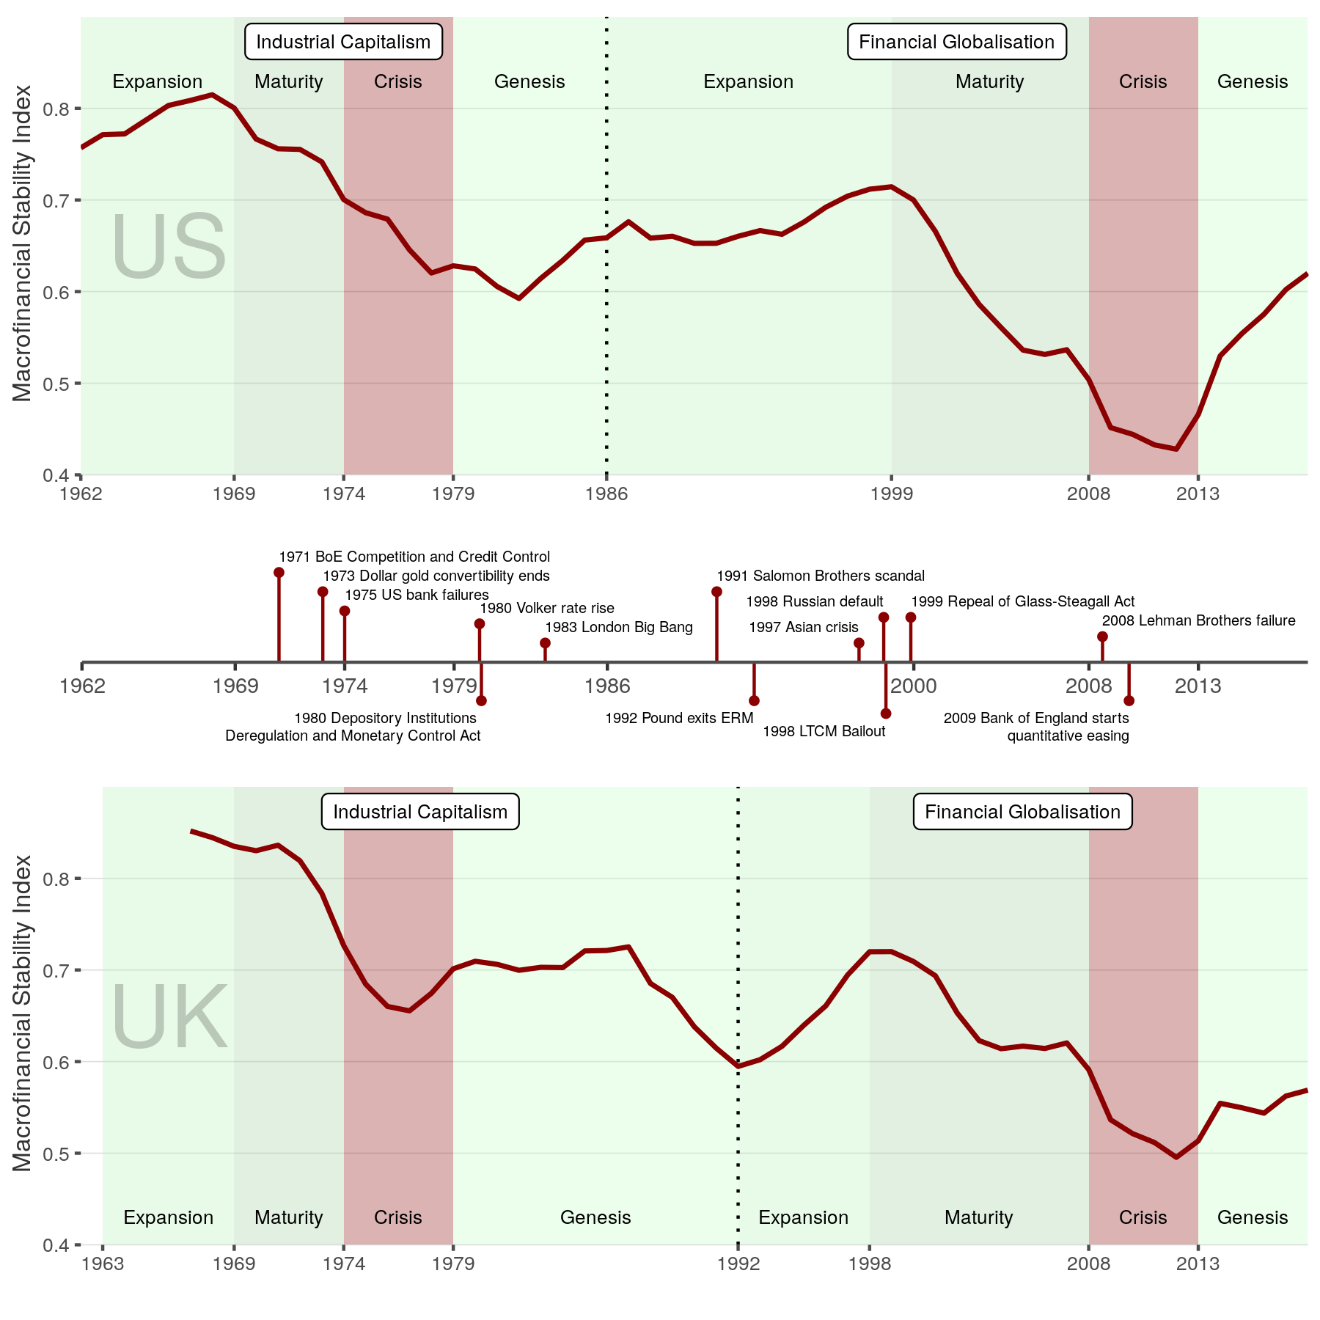
\includegraphics{fig/msi.png}

High-income countries experienced common secular cyclical movements in their
macrofinancial stability in the post-World War II period.

The ideological shift on macroeconomic management at the end of the 1970s brought independent
central banks oriented to inflation targeting and fiscal deficits financed on sovereign debt markets.
Mass privatisation reduced the state's economic footprint, while previous gains on employment
protection and unemployment benefits were substantially rolled back. Growth
increasingly relied on rapid expansion of leverage and increasing financial activity.
The financial sector, in turn, found that new institutional structures were required
to enable leverage to expand beyond traditional constraints.
During the expansionary phase of the FG supercycle, shadow banking expanded significantly,
absorbing the flow of assets resulting from the continued expansion of credit.
Securitisation and the originate-to-distribute model allowed banks to
transform illiquid assets, mortgage loans in particular, into marketable securities.
These securities were financed with short-term liabilities such as
repos and asset-backed commercial paper (ABCP).
Growth became increasingly reliant on collateral-based financial activity.

Collateral plays a central role in funding neorentier balance sheets.
Neorentiers issue short-term (often overnight) repo deposits secured by tradable collateral.
For lenders such as institutional cash pools or money market funds, collateral
makes repos a better liquidity management vehicle than unsecured bank deposits.
Repo borrowing allows a wide range of institutions to access money market
funding, while rising asset prices lead to increasing leverage capacity
because repo collateral is marked to market.
The use of collateral functionally, and imperfectly, replaces direct
sovereign guarantees on short-term liquid assets.

The rise of collateral-based finance fundamentally changed the relationships
between central banks and governments.
In the 1990s, central banks in high-income countries collectively sanctioned neorentiers'
turn to shadow deposits by liberalising repo markets,
often to enable Ministries of Finance to develop liquid government bond markets.
States turned to neorentiers in the age of
independent central banks and capital market financing of budget deficits, introducing reforms in
sovereign bond markets designed according to neorentier preferences:
regular auctions facilitated by primary dealers and deregulated repo markets

The promise of liquidity for sovereign bonds entrenches the `infrastructural power' of finance:
neorentiers promise liquidity to Ministries of Finance, and well-functioning monetary
transmission mechanisms to central banks, improving their ability to oppose policy innovations or
tighter regulatory measures.
The rising power of neorentiers thus serves to discipline
states, curbing fiscal and regulatory thwarting mechanisms:
market financing of fiscal deficits privileges neorentiers as mediators
between the monetary and the fiscal arms of the state, and
creates conflicting objectives for the central bank and the Treasury.

Easy credit conditions allowed sustained expansion of private debt,
enabling aggregate demand to keep up with productive capacity
in the face of weak income growth and government retrenchment.
Credit-financed consumption took over from capital investment as the driver of growth.

While crisis-era innovations succeeded in preventing financial system collapse and depression,
growth has not returned.
In our framework, this less due to `secular stagnation' than to the
institutional architecture of the FG supercycle --
weak and `flexible' labour, high inequality and government retrenchment.
Without a change in this architecture -- without a new set of thwarting mechanisms --
it is difficult to identify a likely source of sustained demand growth other than
a return to credit expansion.

Overall, while institutional changes improved the effectiveness of stabilising mechanisms
in the period prior to the coronavirus pandemic, the continuous push for asset-based welfare
reinforced the structural drivers of neorentier capitalism
without delivering a new engine of growth.
When the coronavirus crisis struck, a new configuration of thwarting mechanisms
that could foster economic expansion alongside financial stability had not yet emerged.
The thwarting mechanisms of the next supercycle will be, at least in part,
the result of the rapid institutional change that has taken place as a result of this crisis,
and of greater awareness of the potential for future pandemics.
Inevitably, the next supercycle will also be conditioned by
the even greater crisis of climate change.

\emph{Green Supercycle}

What is most urgently required, in light of the COVID-19 and
climate crises, is a detailed understanding of the current genesis phase
and the prospects for the emergence of a new set of thwarting mechanisms
that would underpin a green supercycle.

\href{https://www.researchgate.net/publication/343472909_Institutional_supercycles_an_evolutionary_macro-finance_approach}{Dafermos Gabor (2020) Institutional Supercycles}
\href{pdf/Dafermos_Gabor_2021_Institutional_Supercycles.pdf}{(pdf)}

\hypertarget{central-banking}{%
\section{Central Banking}\label{central-banking}}

\emph{Braun}

The impact of international economic integration on social protection is conditional on
the monetary regime.

The role of the European Central Bank (ECB) as the supranational enforcer of the
economic logic of integration since monetary union.

While Polanyi conceptualized central banking as an institution of
non-market coordination that evolved to protect the
domestic economy from gold standard pressures,
the ECB has acted as an enforcer of disembedding ``euro standard'' pressures
vis-à-vis national labor market and welfare state institutions.

Despite lacking the mandate or the authority to override national legislation,
the ECB, strategically pursuing its organizational and systemic interests, pushed
for structural reforms via discursive advocacy and conditionality.
Our results show that
Europe's prospects for Polanyian non-market coordination are determined by Frankfurt
as much as by Luxembourg and Brussels.

\textbf{The death of `Social Europe'}

The European Commission's slogan of ``a Europe that protects'', introduced in 2019,
subtly diverges from the Treaty of Rome's commitment to ``proper social protection.''
This is no accident.
The euro area debt crisis accelerated labor market deregulation and
welfare state retrenchment, and the idea of a ``Social Europe'' has been declared ``dead.''
At the same time, and particularly among those most affected by by these developments,
protectionist and nationalist sentiments have been on the rise.
Brussels watchers have read ``a Europe that protects'' as a bellwether
of a new, non-liberal politics of protection.

The European Union (EU) as a unique case combining
high levels of protection with full
``globalization in the strict sense of the word'',
namely unrestricted competition for capital, goods and services.

The strictures of the euro considerably amplified the economic
logic of integration relative to the legal and political logics
expressed through the ECJ and the Commission, respectively.
With the introduction of the euro in 1999, this economic
logic of integration found its institutional expression in
the European Central Bank (ECB).
Since then, the relationship between economic integration and
social protection has been shaped in Frankfurt as much as in Brussels and Luxembourg.

\textbf{Structural Reforms}

The ECB defined structural reforms, in strikingly Polanyian terms, as policies
that ``change the fabric of an economy, the institutional and regulatory framework in
which businesses and people operate.''

This advocacy constitutes a puzzle:
The ECB lacks both a mandate and the legal means to
shape labor market and social policies
at the member-state level.
Pushing to ``change the fabric'' of societies therefore entails significant
reputational risks.
Why, then, did the ECB chose to push for structural reforms?
Our explanatory framework places the emphasis on
the ECB's organizational (credibility and legitimacy) and
systemic (survival of the euro) interests.
In pursuing those interests, the ECB strategically adjusted the method and content of
its structural reform advocacy to fit the economic and political context.
In the wake of the euro area debt crisis, the
ECB acquired the power---shared with the Commission and the International Monetary
Fund (IMF)---to impose and enforce policy conditionality.

\textbf{Polanyi}

Our analysis, while drawing on Polanyi, fills an important gap in Polanyian thinking
on the political economy of central banking. According to Polanyi, national central bank-
ing evolved as an expression of the countermovement to the commodification of money
under the international gold standard. Whereas Polanyi said little about potential con-
flicts between non-market coordination in the domain of money (central banks) and social
protection in the domain of labor (social policies and trade unions), this conflict subse-
quently moved to the very center of macroeconomic governance.
A large literature has
since studied the interaction between national central banks and national labor market
policies and wage-setting actors.

The institutional setting of this interaction
changed dramatically with EMU, which established a supranational monetary regime with
its own supranational central bank. From the beginning, heterogeneous labor market in-
stitutions and social policies threatened divergent national inflation developments, which
clashed with the ECB's one-size-fits-all monetary policy.

Whereas Polanyi would have
expected a central bank to protect national economies from the disembedding pressures
of the monetary regime, the ECB has instead embodied these very pressures, acting as
a---if not the---key planner of laissez-faire in national labor markets.

Looking beyond Europe, our analysis contributes to the literature on policy diffusion in
the context of economic globalization.
Here, national policymakers routinely encounter
the problems of translating and enforcing perceived functional pressures emanating from
the international level.

The IMF,
guided by the ``Washington Consensus,'' made its emergency lending conditional on gov-
ernments' implementing specific structural reforms, playing the role of both translator
and enforcer.

Central banks, as the ultimate repositories of ``epistemic authority'' on
economic matters, are uniquely positioned to play a similar role at the domestic level.
In the euro area, the role of translator and---to a lesser but significant
extent---enforcer of perceived functional pressures was assumed by the ECB
ECB identified---and sought to counter via structural reforms
and public-sector wage restraint---the diverging trend in unit labor costs
as early as 2005, years before the European Commission.

The ECB has been a highly articulate proponent of specific structural reforms
in national labor markets and social policy regimes.
When unit labor cost divergence, first recognized and prioritized by Trichet,
threatened the very effectiveness of supranational monetary policy, the ECB began to pro-
mote structural reforms as means of macroeconomic adjustment, both in public speeches
and behind the scenes with national policymakers.
Executive Board members urged gov-
ernments to seek downward wage adjustments, both via structural labor market reforms
and by imposing wage restraint on the public sector.
When the euro-area debt crisis hit,
the ground for its interpretation as a crisis of competitiveness divergence had already been
prepared by the ECB.
When circumstances added formal and informal conditionality to
the ECB's toolkit, it wielded those instruments to help \emph{enforce}
labor market liberalization, internal devaluation, and public sector wage cuts.
It was only when deflationary pressures
and criticism in the European Parliament and elsewhere threatened its legitimacy that
the ECB abandoned its advocacy of structural reforms.

Despite lacking both a mandate and the legal
means to directly override national regulations, the ECB has been a keen supranational
advocate of market-enhancing integration in the field of labor market and social policy.

This analysis also sheds new light on the broader political economy of central banking.
Polanyi and others have shown that national central banking evolved under the interna-
tional gold standard to buffer the disruptive adjustment pressures on national economies.
The supranational ECB provided such protection for the financial system, but not for
labor. Instead, emulating the role the IMF in other parts of the world, the ECB trans-
lated---and subsequently helped to enforce---the perceived functional pressures of interna-
tional monetary and financial integration. Whether the ECB is constitutionally wedded
to the role of ``prime mover in the move to a market society'' remains to be seen. 135 Its
recent shift from structural reform advocacy to calls for wage increases has been echoed
in the US, where the Federal Reserve has signaled that it will prioritize employment and
wage growth over consumer and asset price stabilization. Central banks may yet again
become ``active agents of the countermovement.''

\href{https://osf.io/preprints/socarxiv/dp3nv}{Braun (2021) Planning Laissez-faire: Supranational Central Banking}
\href{pdf/Braun_2021_Planning_laissez-faire.pdf}{(pdf)}

\hypertarget{externalities}{%
\chapter{Externalities}\label{externalities}}

Resource extraction and pollution of the commons
power the beating heart of global economic prosperity.

\hypertarget{history-of-economics-externalities}{%
\section{History of Economics' `Externalities'}\label{history-of-economics-externalities}}

\emph{Duncan Austin}

\textbf{Incomplete Markets}

Externalities were generally ignored through most of the 20 Century. After Pigou had
identified the problem in the 1920s, there followed a long barren period for ``welfare
economics'', the natural home for this type of thinking. This lasted until the early 1970s when there were the first stirrings of renewed interest by serious economists.

Framed as ``externalities'', market failures could be more easily dismissed.
The term encourages a perception of unpriced damages as
being mere residuals to the centrepiece of a priced economy.
Since Pigou, some have sought to ``beef up'' the terminology.
K. William Kapp, for example, bluntly described the market mechanism, in toto,
as a ``cost-shifting'' institution.
In this framing, externalities are not a bug, but a feature.

The mathematization of economics -- another marker of the discipline's
scientific aspiration -- exacerbated the situation.
The desire for manageable equations and functioning models
further pushed troublesome market imperfections away.
Possibly, there was the sense that positive and negative externalities
might roughly cancel each other out, leaving GDP incomplete
but still reliable enough as a directional indicator.
That rests on the assumption that positive and negative externalities are
symmetrical in nature.

However, there is an important asymmetry.
Positive externalities take the form of ``free goodies'', whereas certain negative externalities constitute systemic risks that
may be catastrophic to ``trip'' or breach. While you generally cannot have too much of a
positive externality -- a ``free good thing'' -- too much of certain unwanted harms may induce
systemic failure.

Externalities exist because markets have an incomplete grasp of what humans value. Markets
work off prices and not everything has -- or can have -- a price. As such, marketed values -- or
prices -- exist amidst a broader ``value field'' of things that humans care about and which have
an influence on our wellbeing.

Pigou's proposition was an inconvenient truth for economics. It suggested that there are real
limits to what conventional economics might say about matters of human value and, hence, to
how far markets might serve human wellbeing. The inconvenience of his idea may be why
Pigou is not better known -- seemingly more tolerated, than celebrated

\textbf{Complete markets\ldots?}

As a discipline, economics did the very human thing of trying to ignore a difficult proposition.
By not confronting Pigou's awkward challenge, the door was opened for a line of theorizing
th
that led in exactly the opposite direction. Economists for most of the 20 Century sought to
establish economics as a comprehensive corpus of thought with universal application.

Hence, by the 1950s, a very appealing theory of complete markets had been developed. No
externalities in this theory, none at all.

Complete market theory is the laying
down of a conceptual blanket over all our preferences that leaves no space for externalities.

The formulation of complete markets theory was deemed a major milestone for economics. Its authors were Kenneth Arrow and Gérard Debreu.
It provided the cornerstone for the discipline's claim for the
superiority of markets as a mechanism for social coordination.

\textbf{Rather, the key mistake made by 20 Century economics was not in misunderstanding
externalities, but in grossly underestimating their magnitude} and
so foreclosing a debateon the innate limits of economic thinking.
The discipline considered that markets were ``complete enough'' to
safely proceed as if they were actually complete!
We are now waking up to the consequences of that misjudgement.

\textbf{\ldots{} Or very incomplete markets?}

Consider, for example, a recent study by Robert Costanza and colleagues. They estimated
the monetary value of the ``services'' provided free by the Earth's ecosystem at \$125 trillion in
2
2011, nearly twice the value of global GDP (gross domestic product) at the time.
The authors believe this to be a conservative estimate because it grasps only about half of the ``services'' we know ecosystems provide.

Other studies have contemplated the value of unmonetized social systems, including one
estimate that unpaid housework in the UK in 2016 was about 65 percent of GDP -- another
3
huge block of value not captured by the market. Just combining this figure with the Costanza
et al.~figure suggests that measured GDP captures about a third of some larger conception of
value.

From its very inception, GDP has been derided as an incomplete measure of wellbeing.
However, in elevating GDP to its current perch of influence, the working assumption has been
that GDP, and the market system it reflects, captures the lion's share of what matters. What
the latest estimates of ``externalities'' and non-market values suggest -- and what our
sustainability crisis seems to underscore -- is that our perception of GDP's reach may be
horribly off. Such an estimate suggests that it is not that the market does not capture \emph{all} things of value, it does not even capture \emph{most} things of value.
\textbf{Far from externalities being peripheral, they may be the main event!}

The failure of economics to fully incorporate externalities in its 20th-century
theorizing now appears to be the dropped stitch that defines the whole discipline. For a long
time, this was a tolerable neglect as markets were more robustly counterbalanced by pre-
market institutions that upheld unpriced values, and as the environment was able to absorb
the fewer demands of a smaller, less consumptive population. But, with the onset of climate
and biodiversity emergencies, the context has changed considerably. It matters more and
more that we might not have \emph{slightly incomplete markets}, but \emph{very incomplete markets}.

It has left us at the start of the 21 Century transforming
the matter and energy of the world using
economic and financial tools that have only
a very limited grasp of the reality they fashion.

In a world of very incomplete markets, things of human value lie in two separate realms -- the
marketed domain and the non-marketed domain. Some of the growth of the marketed
economy genuinely arises from human ingenuity and creativity unlocking better ideas and
products from new combinations of inputs. This is ``good'' growth, which ought to be
celebrated and encouraged. However, other parts of monetized ``growth'' arise from simply
running down the stocks of what is valuable but in the non-marketed realm. This is the illusion
of wealth creation based on registering the increase in marketed value, but not recording the
decrease in unmarketed values. In contrast to growth from genuine ingenuity, this is robbing
Peter to pay Paul.

Measured economic ``growth'' overall combines in unknown proportions a ``creative
growth'', which we want to encourage, and a ``parasitic growth'', which we do not. At an
aggregate level, it is almost impossible to trace the origins -- creative or parasitic -- of GDP
growth, and very few official metrics make any attempt to do so.

Our working assumption is that all
economic growth is good -- as it indeed would be if we had complete markets eliminating the
possibility of parasitic growth. However, in not knowing the real-world mix between creative
and parasitic growth, do we want more GDP growth, or less? It is not clear. And, given that
companies work to the same price register as GDP, do we want companies to beat profit
expectations or would it be better if they missed them? Who really knows?
The conventional argument -- captured by the notion of an Environmental Kuznets Curve -- is
that it is only by increasing monetary wealth that we can develop better technology to protect
the environment. However, it is not clear in the aggregate whether the deployment of such
new capabilities ever makes good the damage done by the initial enabling wealth creation.
While anecdotes can be summoned to support the idea -- electric cars, wind turbines, LEDs
etc -- thus far, at the global level that matters, data shows we remain in net ecological
destruction mode.

\textbf{Markets within Cultures}

Paradoxically, then, to use markets more than we are, to introduce more externality pricing,
would require a new cultural level reassertion that markets are a tool within culture. We need
not a sustainable economy, but a sustainable culture that has an economy. Such a culture
would establish room for governments to introduce new markets which powerful market
ncumbents may not like, but which improve human wellbeing. In turn, such a culture would
also invigorate non-market means to protect our environment, for we must remember that not
everything of human value can be priced and ``internalized''. The interesting question, worth a
moment's reflection, is: why is that?

\textbf{Commodifiable Externalities}

Though Pigou identified commodifiable externalities, there are many things of human value
that cannot withstand the disembedding from their context necessary for them to be
commodified and, hence, be transactable via market exchange. Such values are non-
transactable because they are irrevocably embedded either in specific things -- they are
unique -- or in specific relations -- they exist ``between'' certain things. Some examples:
friendship, reputation, loyalty, integrity, trust, community, mental health, etc. If you believe you
have purchased any of these items, you might want to check the label.

What is tricky is that most things in the world bear both separable transactable values and
intrinsic non-transactable values. A tree has both separable value as a feedstock for furniture
and paper and intrinsic value as part of the ecosystem in which it is relationally embedded.

We tend to value trees in managed plantations for their separable values, but we value
General Sherman, the 26-story-tall giant sequoia that is the largest known tree on Earth, for
its non-separable attribute of being uniquely the tree we call General Sherman.
With General Sherman, we have chosen to perceive and value its uniqueness over its
instrumental value. Indeed, we might say that General Sherman is price-less. The
``economist'' denies the validity of this perspective by arguing that everything has a price. To
say that something is priceless is merely to say that nobody has yet offered a high enough
price.
In turn, the ``ecologist'' denies the ``economist's'' perspective, arguing that while you can apply
such economic thinking to General Sherman, it is the wrong sort of thinking to apply.

Both the ``economic'' transactional perspective and the ``ecological'' intrinsic perspective are
beneficial and valid, but they are incompatible.

The decision to
apply an economic perspective to the external world is always a value judgment that
necessarily transcends economics. More, it is a value judgment that can never be justified or
refuted on economic grounds precisely because it is an argument about the validity of
applying an economic perspective.

All this is a discussion that the field of economics may well have taken more seriously 100
years ago, had it been more open to the significance and implications of Pigou's formulation
of externalities. Alas, we are now having to unknit to pick up this dropped stitch in a world now
confronting large-scale problems of missed externalities.

\textbf{Incompletness Theorem of Economics}

Economics might be well served by formalizing an incompleteness theorem that would act as
a proverbial knot-in-a-handkerchief reminder about the limits of claims that economics can
make. It is an oddity of human intellectual thought that the most logical of our sciences,
mathematics, had a formal Incompleteness Theorem as early as 1930, while economics
formalized a complete market theory in the 1950s and seemingly still has no definitive
statement of incompleteness.

\textbf{Ringfecing Economics}

One of the ways, then, that we could better protect ecological values is for economics to
recognize -- re-cognize -- the wisdom of culturally ring-fencing where economic thinking is
preferred. In other words, to recognize the non-monetizable value of non-economic thinking.

Designating areas as protected are to explicitly restrain the ever-eager economic perspective.
Such boundaries need to be upheld at the social or cultural level to count for anything.
If not individuals can always free ride and extract the monetary instrumental value
that others have agreed not to pursue.

While economics is undoubtedly \emph{a} valuable form of knowledge, it is a way of seeing things,
not \emph{the} way.

A full century after Pigou formalized the idea of externalities, we might mark the
anniversary by taking more seriously the effort to clarify the appropriate reach of economics
and markets within the broader social and cultural context.

\textbf{Economics is about solved Political Problems}

Arguably, one of the most important questions in economics is not even an economic
question.
The field effectively punts the matter of its own ontology -- the things that economics
can talk about -- to a different discipline. In Abba Lerner's words:

\begin{quote}
``An economic transaction is a solved political problem. Economics has
gained the title of Queen of the Social Sciences by choosing solved political
problems as its domain.''
\end{quote}

Economics has been strangely content to focus its efforts on pattern-seeking within a domain
it leaves other disciplines to define, but in the absence of contemplating its boundaries more
explicitly, it has hubristically come to believe it has greater reach than it really has.

In turn, this leaves most economists -- and the great many people who think and act
economically in conducting their professional duties -- dangerously unaware of where
economic thinking is beneficial and valid and where it ultimately hits limits.

\href{pdf/Austin_2021_Pigou_and_the_dropped_stitch_of_economics_RWER95.pdf}{Duncan Austin: Pigou and the dropped stitch of economics RWER95 (pdf)}

\hypertarget{ecosystem-services}{%
\section{Ecosystem Services}\label{ecosystem-services}}

\emph{Constanza}

• Global loss of ecosystem services due to land use change is \$US 4.3--20.2 trillion/yr.
• Ecoservices contribute more than twice as much to human well-being as global GDP.
• Estimates in monetary units are useful to show the relative magnitude of ecoservices.
• Valuation of ecosystem services is not the same as commodification or privatization.
• Ecosystem services are best considered public goods requiring new institutions.

In 1997, the global value of ecosystem services was estimated to average \$33 trillion/yr in 1995 \$US (\$46 trillion/yr in 2007 \$US). In this paper, we provide an updated estimate based on updated unit ecosystem service values and land use change estimates between 1997 and 2011. We also address some of the critiques of the 1997 paper. Using the same methods as in the 1997 paper but with updated data, the estimate for the total global ecosystem services in 2011 is \$125 trillion/yr (assuming updated unit values and changes to biome areas) and \$145 trillion/yr (assuming only unit values changed), both in 2007 \$US. From this we estimated the loss of eco-services from 1997 to 2011 due to land use change at \$4.3--20.2 trillion/yr, depending on which unit values are used. Global estimates expressed in monetary accounting units, such as this, are useful to highlight the magnitude of eco-services, but have no specific decision-making context. However, the underlying data and models can be applied at multiple scales to assess changes resulting from various scenarios and policies. We emphasize that valuation of eco-services (in whatever units) is not the same as commodification or privatization. Many eco-services are best considered public goods or common pool resources, so conventional markets are often not the best institutional frameworks to manage them. However, these services must be (and are being) valued, and we need new, common asset institutions to better take these values into account.

\href{https://doi.org/10.1016/j.gloenvcha.2014.04.002}{Constanza (2014) Global value of ecosystem services (Paywall)}
\href{pdf/Costanza_2014_Global_Ecosystem_Services.pdf}{(pdf)}

\href{pdf/Costanza_2019_Natural_Capital_and_Ecosystem_services.pdf}{Constanza (2019) Natural Capital and ERcosystem Services}

``The fossil fuel industry has been granted the greatest market subsidy ever: the privilege to dump its waste products into the atmosphere at no charge.'' (Michael Mann)

\hypertarget{environmental-degradation}{%
\section{Environmental Degradation}\label{environmental-degradation}}

\hypertarget{kuznets-and-engel-curves}{%
\subsection{Kuznets and Engel Curves}\label{kuznets-and-engel-curves}}

\emph{Environmental Kuznets and Engel's Curve}

I think degrowth is wrong on the merits (environmental kuznets curves and environmental engel curves
are both concave),
but it's also an obvious nonstarter even if it was founded on solid footing,
To spell this out: if EKC and EECs are concave,
redistribution within or between countries doesn't necessarily reduce environmental damages.
(John Voorheis (twitter))

\emph{Abstract Maneejuk:}

This study aims to examine the relationship between economic development and
environmental degradation based on the Environmental Kuznets Curve (EKC) hypothesis. The level
of CO 2 emissions is used as the indicator of environmental damage to determine whether or not greater
economic growth can lower environmental degradation under the EKC hypothesis. The investigation
was performed on eight major international economic communities covering 44 countries across
the world. The relationship between economic growth and environmental condition was estimated
using the kink regression model, which identifies the turning point of the change in the relationship.
The findings indicate that the EKC hypothesis is valid in only three out of the eight international
economic communities, namely the European Union (EU), Organization for Economic Co-operation
and Development (OECD), and Group of Seven (G7). In addition, interesting results were obtained
from the inclusion of four other control variables into the estimation model for groups of countries
to explain the impact on environmental quality. Financial development (FIN), the industrial sector
(IND), and urbanization (URB) were found to lead to increasing CO 2 emissions, while renewable
energies (RNE) appeared to reduce the environmental degradation. In addition, when we further
investigated the existence of the EKC hypothesis in an individual country, the results showed that the
EKC hypothesis is valid in only 9 out of the 44 individual countries.

\href{https://www.google.com/url?sa=t\&rct=j\&q=\&esrc=s\&source=web\&cd=\&cad=rja\&uact=8\&ved=2ahUKEwibz9unoJHvAhVPXRoKHeUDC5sQFjAIegQIBxAD\&url=https\%3A\%2F\%2Fwww.mdpi.com\%2F2071-1050\%2F12\%2F21\%2F9117\%2Fpdf\&usg=AOvVaw35OuEm4BhDFbPAb_esW2hF}{Maneejuk (2020) Does the Environmental Kuznets Curve Exist?}
\href{pdf/Maneejuk_2020_Does_EKC_exist.pdf}{(pdf)}

The Kuznets curve expresses a hypothesis advanced by economist Simon Kuznets in the 1950s and 1960s.
\textbf{As an economy develops, market forces first increase and then decrease economic inequality.}

Since 1991 the environmental Kuznets curve (EKC) has become
a standard feature in the technical literature of environmental policy,
though its application there has been strongly contested.

The environmental Kuznets curve (EKC) is a hypothesized relationship between environmental quality and
GDP growth:
according to its argument, which is spurious,
various indicators of environmental degradation tend to get worse as modern economic growth occurs
until average income reaches a certain point over the course of development,
at which point some studies have argued, they improve.

It first became popular as introduced by Gene Grossman and Paul Krueger in their working paper:
``Environmental Impacts of a North American Free Trade Agreement.''
This paper simply showed that the non-direct Greenhouse gas, Sodium Dioxide, Dark Matter,
and Suspended particles followed an inverted-U shaped pattern.
This was almost immediately misinterpreted by the World Bank and Beckerman and
adopted into policy as an argument that all negative environmental effects would follow an EKC pattern.
Copious research has concluded that beyond these pollutants, and issues like water quality,
that immediately threaten human health,
GDP growth essentially harms, and does not help the environment with no lasting ``turning point.''
The EKC has led to poor policy choices reaping untold environmental damage.

\href{https://en.wikipedia.org/wiki/Kuznets_curve\#Environmental_Kuznets_curve}{Wikipedia}

\hypertarget{energy-and-transport}{%
\section{Energy and Transport}\label{energy-and-transport}}

The ``hidden cost'' of our largely fossil fuel-based energy and transport systems could add up to around \$25 trillion (£18 trillion) -- the equivalent of more than a quarter of the world's entire economic output.

That's according to new research, which estimates the hidden environmental, social and health costs associated with different forms of transport and electricity generation.

\href{https://www.sciencedirect.com/science/article/pii/S2214629620304606}{Sovacol (2021)}
{[}(pdf){[}(pdf/Sovacol\_2021\_Energy\_and\_Transport\_Externalities.pdf)

\href{https://www.independent.co.uk/climate-change/news/energy-transport-cost-fossil-fuels-b1805808.html}{Independent}

\hypertarget{money}{%
\chapter{Money}\label{money}}

\hypertarget{inflation}{%
\section{Inflation}\label{inflation}}

Monetarist theory, which came to dominate economic thinking in the 1980s and the decades that followed, holds that rapid money supply growth is the cause of inflation. The theory, however, fails an actual test of the available evidence. In our review of 47 countries, generally from 1960 forward, we found that more often than not high inflation does not follow rapid money supply growth, and in contrast to this, high inflation has occurred frequently when it has not been preceded by rapid money supply growth.

There are several implications. The most relevant of these seems to be that the current efforts of central banks to engender inflation are unlikely to be successful.

Based on our examination of countries that together constitute 91 percent of world GDP, we suggest that high inflation has infrequently followed rapid money supply growth, and in contrast to this, high inflation has occurred often when it has not been preceded by rapid money supply growth. The U.S. economy may well experience some increase in inflation in the coming year, but if it does, it is likely it will be due to factors other than monetary policy.

\href{https://evonomics.com/moneysupply/}{Money Growth Inflation}

\hypertarget{fed-policy-and-inflation}{%
\subsection{FED Policy and Inflation}\label{fed-policy-and-inflation}}

When you view money supply and velocity together, one notices they tend to offset each other. However, we highlight the late 1970s, the last highly inflationary period, to show a period they did not counteract each other.

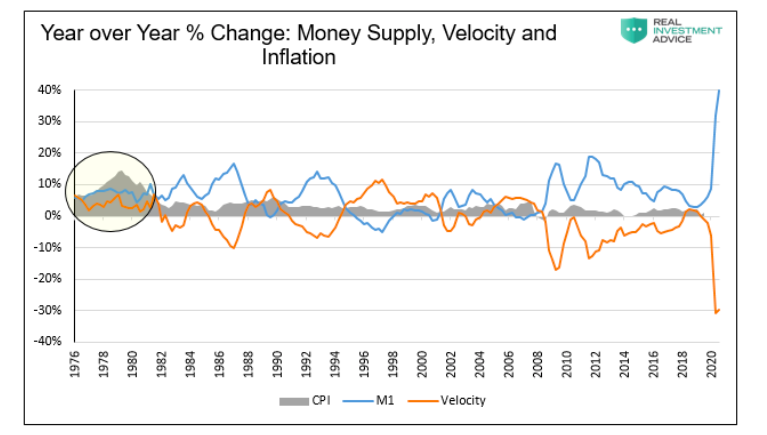
\includegraphics{fig/money_and_inflation_US.png}

The Fed and Treasury are playing a dangerous game. The numbers we discuss above are massive and dwarf anything seen in American history. If consumers start spending their savings, and the government keeps borrowing and spending unprecedented amounts, velocity can pick up rapidly. We leave you with a vital question to better understand the prospects for inflation.

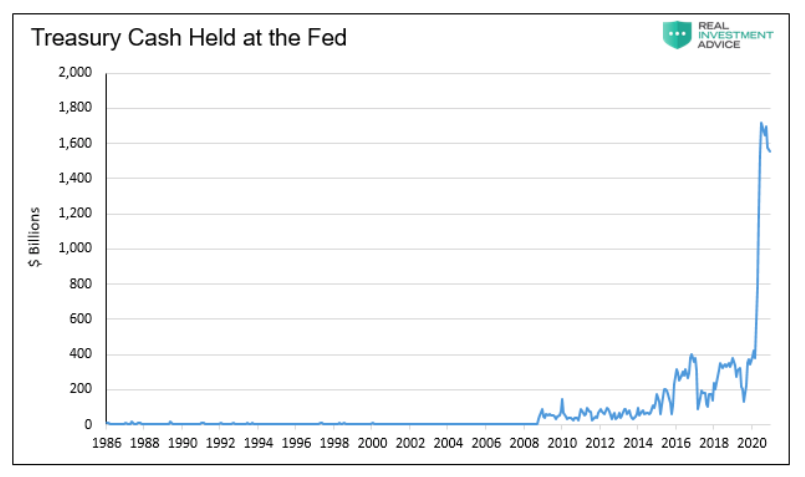
\includegraphics{fig/Treasury_cash_at_FED.png}

\href{https://www.seeitmarket.com/is-inflation-coming-in-2021-watch-money-supply-and-velocity/}{Lebowitz}

\href{https://realinvestmentadvice.com/stoking-the-embers-of-inflation/}{Lebowitz and Freeze}

\hypertarget{modern-monetary-theory-mmt}{%
\section{Modern Monetary Theory (MMT)}\label{modern-monetary-theory-mmt}}

\emph{Culbreath}

The common conservative objection to government spending is not only based on a faulty economic model, but it also serves as a mental obstacle to using government capacity for purposes conservatives are supposed to care about.

Conservatives should re-examine the economics that underlie the tendency on the right to condemn any instance of large-scale government spending.
The policy conversation could then shift away from whether government spending is economically justifiable and towards what kinds of spending are productive and worthwhile.

According to MMT, no sovereign state that issues its own currency can ever run out of money. This is because it simply ``prints'' its money in order to pay for whatever operations it deems necessary. The government doesn't need to go out and find the money it needs for such spending; it needs no fundraisers, no sales, and not even taxes, to fund its operations. It simply spends into existence the money that it needs for its operations.

unlike any private entity, such as a household or a corporation, the government does not need to worry about its own solvency, since it can never go insolvent---it can never run out of money. Thus, the government does not need to take any of the measures that private entities take to accumulate savings or make a profit. It will always be able to ``spend into existence'' whatever money it needs to pay for its operations. The difference between the federal government and a household is thus not merely a difference in degree (one is bigger than the other). It is a difference in kind.

It follows that taxes do not amount to the accumulation of wealth for the government. Rather, they amount to no more than the extinction of money from the economy. Like God, the government giveth, and the government taketh away; the government spends money into the economy by printing it and removes money from the economy by taxing it.

In terms of the pure quantity of government spending, there is no limit except inflation to what the government may spend. Inflation only occurs, at least in any damaging degree, under certain conditions. Foremost among those conditions is full employment. When the economy is at full employment, which it rarely is, then the overall purchasing power within the economy may be considered to be at full capacity. At this point, an injection of more money into the economy might result in inflation, since it would likely push demand to outstrip supply, thereby causing prices to soar higher and purchasing power to decline at a dangerous rate.

However, even this danger could be averted to a significant degree if the government aimed its spending not only at stimulating demand but also at stimulating the production of consumer goods. In fact, the U.S. government has a long history of doing exactly this, as the extensive research of economists like Mariana Mazzucato demonstrates quite compellingly. If there is a risk of inflation from government spending, it would not be because government spending automatically produces inflation. Rather, it might be due to the fact that the U.S. government has ever since the Reagan era failed to make a priority of stimulating both demand and production through the implementation of a deliberate industrial policy. This only highlights further the importance of well-planned spending by the government.

Furthermore, the government has many other tools at its disposal for controlling inflation. Not only does the Federal Reserve play a central role here, but even taxes can be levied by the government as a way of controlling inflation. When demand begins to outstrip supply, the government may very well consider imposing taxes where this might effectively limit inflation. Of course, not just any taxation would do this; the government needs to ensure that its taxes target entities or classes who spend enough money to affect consumer prices. Taxing the extremely wealthy, for example, may not be the best way to control inflation, since wealthy people tend to save more than they spend.

while there are many good reasons for the government to impose taxes, especially to control inflation, funding government expenditure is not one of those reasons. Indeed, the idea that taxes should fund the government's expenditure by ``plugging its deficits'' could prove to have damaging effects on the economy as a whole, if actually put into practice. As MMT theorists are fond of pointing out, what we call the government's deficit actually amounts to nothing other than the people's surplus.

As long as the government (public sector) spends more into the economy (private sector) than it taxes out (the definition of deficit spending), the economy itself will enjoy a money supply large enough to stimulate productivity and growth. By contrast, if the government were to tax more out of the economy than it spent into it, the economy would suffer from its own deficit, a risk of deflation, and a potential crisis of underconsumption. In other words, the deficit by itself is not a bad thing, and it is here to stay.

\href{https://www.theamericanconservative.com/articles/modern-monetary-theory-for-conservatives/}{Culbreath (2021) MMT for Conservatives}

\hypertarget{markets}{%
\chapter{Markets}\label{markets}}

\hypertarget{markets-as-entropy-maximisers}{%
\section{Markets as Entropy Maximisers}\label{markets-as-entropy-maximisers}}

Markets are randomising machines,
they maximise entropy,
and this fact alone is sufficient to explain some of the inequality we observe.

Market transactions involve a transfer of monetary value. After any transaction one party may have more or less money than before.

It's quite easy to write a short simulation program that takes a large collection of individuals that start with equal amounts of money. We then pick two individuals at random. One is the buyer. We randomly choose a proportion of their money to spend. The seller gets that money. We then repeat, and pick another two individuals at random. And we keep doing this forever.

After a short period, we can then measure the distribution of money across individuals. And we find, once again, the exponential distribution. Most individuals have very little money, and a small number have a great deal.

So the activity of market exchange is acting just like the cocktail shaker: its mixing everything up, randomising things, and maximising the entropy of the system.

You might think that this model of money exchange is far too simple to tell us anything about real markets. But you'd be wrong.

Remarkably, we observe the exponential distribution in actual economies. The exponential is a great fit to the bottom 80\% of the wealth distribution, which is the vast majority of the population. And this holds true for whichever capitalist country we look at.

The fact that 80\% of the wealth distribution of actual economies follows an exponential law is a very astonishing regularity.

We might think that differences in wealth must arise from accidents of birth or personal virtue. But the principle of entropy maximisation tells us there's a much more important causal factor at work. We quickly get extreme income inequality even in an economy with identical individuals with identical initial endowments of money.

The points is that markets are randomising machines, they maximise entropy, and this fact alone is sufficient to explain some of the inequality we observe.

So the anarchy of the market is the primary and essential cause of economic inequality.

\begin{quote}
But why doesn't the exponential law fit the entire wealth distribution?
What about the remaining 20\% of rich people?
\end{quote}

\hypertarget{the-social-relations-of-production-as-constraints}{%
\subsection{The social relations of production as constraints}\label{the-social-relations-of-production-as-constraints}}

\href{https://ianwrightsite.wordpress.com/2017/11/16/the-social-architecture-of-capitalism/}{Ian Wright}

\hypertarget{demand}{%
\chapter{Demand}\label{demand}}

\hypertarget{human-needs}{%
\section{Human Needs}\label{human-needs}}

I remember being fascinated when I discovered Manfred Max-Neef's matrix of human needs. It's such a rich description of the human animal that defies reduction to a single dimension. It puts homo economicus to shame. (Blair Fix)

\href{https://t.co/OIXQbLvM0z?amp=1}{Manfred Max-Neef (2007) Development and Human Needs}
\href{pdf/Manfred_Max-Neef_2007_Fundamental_Human_Needs.pdf}{(pdf)}

\hypertarget{aggregate-demand-function}{%
\section{Aggregate Demand Function}\label{aggregate-demand-function}}

Since 1976, Robert Lucas---he of the confidence that the ``problem of depression prevention has been solved''---has dominated the development of mainstream macroeconomics with the proposition that good macroeconomic theory could only be developed from microeconomic foundations. Arguing that ``the structure of an econometric model consists of optimal decision rules of economic agents'' (Lucas, 1976, p.~13), Lucas insisted that to be valid, a macroeconomic model had to be derived from the microeconomic theory of the behaviour of utility-maximizing consumers and profit-maximizing firms.

In fact, Lucas's methodological precept---that macro level phenomena can and in fact must be derived from micro-level foundations---had been invalidated before he stated it. As long ago as 1953 (Gorman, 1953), mathematical economists posed the question of whether what microeconomic theory predicted about the behaviour of an isolated consumer applied at the level of the market. They concluded, reluctantly, that it did not:

\begin{quote}
Market demand functions need not satisfy in any way the classical restrictions which characterize consumer demand functions\ldots{} The importance of the above results is clear: strong restrictions are needed in order to justify the hypothesis that a market demand function has the characteristics of a consumer demand function. Only in special cases can an economy be expected to act as an `idealized consumer'. The utility hypothesis tells us nothing about market demand unless it is augmented by additional requirements.' (Shafer and Sonnenschein, 1993, p.~671-72)
\end{quote}

What they showed was that if you took two or more consumers with different tastes and different income sources, consuming two or more goods whose relative consumption levels changed as incomes rose (because some goods are luxuries and others are necessities), then the resulting market demand curves could have almost any shape at all. They didn't have to slope downwards, as economics textbooks asserted they did.

This doesn't mean that demand for an actual commodity in an actual economy will fall if its price falls, rather than rise. It means instead that this empirical regularity must be due to features that the model of a single consumer's behaviour omits. The obvious candidate for the key missing feature is the distribution of income between consumers, which will change when prices change.

The individual demand curve is derived by assuming that relative prices can change without affecting the consumer's income. This assumption can't be made when you consider all of society---which you must do when aggregating individual demand to derive a market demand curve---because changing relative prices will change relative incomes as well.

Since changes in relative prices change the distribution of income, and therefore the distribution of demand between different markets, demand for a good may fall when its price falls, because the price fall reduces the income of its customers more than the lower relative price boosts demand.

The sensible reaction to this discovery is that individual demand functions can be grouped only if changing relative prices won't substantially change income distribution within the group.

Alan Kirman proposed such a response almost 3 decades ago:

\begin{verbatim}
If we are to progress further we may well be forced to theories in terms of groups who have collectively coherent behavior. Thus demand and expenditure functions if they are to be set against reality must be defined at some reasonably high level of aggregation. The idea that we should start at the level of the isolated individual is one which we may well have to abandon. (Kirman, 1989, p. 138)
\end{verbatim}

Unfortunately, the reaction of the mainstream was less enlightened: rather than accepting this discovery, they looked for conditions under which it could be ignored. These conditions are absurd---they amount to assuming that all individuals and all commodities are identical. But the desire to maintain the mainstream methodology of constructing macro-level models by simply extrapolating from individual level models won out over realism.

\textbf{Macroeconomics cannot be derived from microeconomics.}

\href{https://evonomics.com/why-economists-have-to-embrace-complexity-steve-keen/}{Steve Keen}

\hypertarget{productivity}{%
\chapter{Productivity}\label{productivity}}

\hypertarget{productivity-pay-gap}{%
\section{Productivity-Pay Gap}\label{productivity-pay-gap}}

Using prices to aggregate `output' leads to bizarre problems. On the one hand, it causes `productivity' to be equivalent to average hourly income. This means that any connection between `productivity' and wages is circular. On the other hand, the same decision causes `productivity' to be ambiguous. Our measure of `productivity' depends on arbitrary choices about how to adjust for price change. As a result, productivity trends (like the one in Figure 1) are riddled with uncertainty.

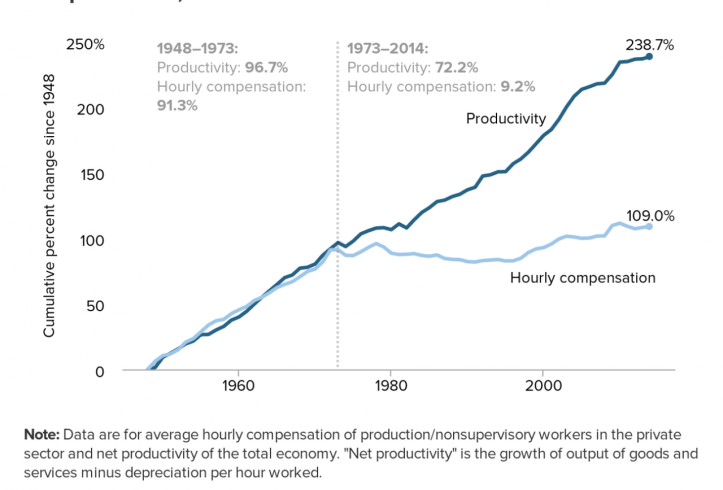
\includegraphics{fig/productivity_pay_gap.png}

`Productivity' is used by both major schools of economic thought. Neoclassical economists use productivity to claim that the distribution of income is just. They argue that in a competitive economy, workers get what they produce. Marxists, in contrast, use productivity to claim that the distribution of income is unjust. They argue that in a capitalist economy, workers receive less than they produce (because capitalists extract a surplus).

What's interesting is that these two opposing theories commit the same sin. They define productivity in terms of income. Neoclassical economists do so explicitly, as I've described in this post. Marxists do so implicitly because they haven't developed their own system of national accounts. Instead, Marxists who do empirical work use neoclassical measures of productivity.

The result of this circular definition is that the analysis of productivity is a sleight of hand. `Productivity' is just income relabelled.

The `productivity-pay gap' is a textbook example of this relabelling. It claims to show a growing gap between what workers `produce' and what they get paid. But workers' `productivity' is actually measured in terms of income --- the average hourly income.

\href{https://economicsfromthetopdown.com/2020/01/17/debunking-the-productivity-pay-gap/amp/}{Blair Fix: Debunking Productivity}

\textbf{Productive individuals, productive society?}

In the 1990s, geneticist William Muir conducted experiments on chickens to see what would
improve egg-laying productivity.
In one trial, he did exactly what the eugenicists recommend -- he let only the most productive hens
reproduce. The results were disastrous. Egg-laying productivity did not increase.
It plummeted. Why? Because the resulting breed of hens was psychopathic.
Instead of producing eggs, these ``uber-hens'' fought amongst themselves, sometimes to the death.

The reason this experiment did not work is that egg-laying productivity is not an isolated
property of the individual hen.
It is a joint property of the hen and her social environment.

In Muir's experiment, the most productive hens laid more eggs not because they were innately
more productive, but because they suppressed the productivity of less dominant chickens.

By selecting for individual productivity, Muir had inadvertently bred for social dominance.
The result was a breed of bully chicken that could not tolerate others.

The lesson here is that in social animals, traits that can be measured among individuals (like
productivity) may not actually be traits of the individual.
Instead, they are joint traits of both the individual and their social environment.
Here is evolutionary biologist David Sloan Wilson reflecting on this fact:

\begin{quote}
``Muir's experiments \ldots{} challenge what it means for a trait to be regarded as
an individual trait. If by `individual trait' we mean a trait that can be measured
in an individual, then egg productivity in hens qualifies. You just count the
number of eggs that emerge from the hind end of a hen. If by ``individual trait''
we mean the process that resulted in the trait, then egg productivity in hens
does not qualify. Instead, it is a social trait that depends not only on the
properties of the individual hen but also on the properties of the hen's social
environment''.
\end{quote}

\href{pdf/Fix_2021_Human_Capital_RWER95.pdf}{Blair Fix: Human Capital Theory RWER95 (pdf)}

\hypertarget{resource-economics}{%
\chapter{Resource Economics}\label{resource-economics}}

\hypertarget{sustainability}{%
\section{Sustainability}\label{sustainability}}

\textbf{`Sustainable Growth' - An Oxymoron}

\emph{Daly Memo}

It is impossible for the world economy to grow it's way out of poverty and
environmental degradation. Sustainable growth is impossible.

In its physical dimanesions the economy is an open sub-system of the Earth ecosystem
which is finite, nongrowing and materially closed.
As the economic sub-system grows it incorporates an even greater proportion
of the total ecosystem into itself and must reach a limit at 100 percent,
if not before.
Therefore its growth is not sustainable.

The term ``sustainable growth'' when applied to the economy is a bad oxymoron -
self-contradictory as prose, and unevocative as poetry.

Sustainable Development (qualitatively) OK
Even `green growth' is not sustainable.

In the past 200years we have developed a culture dependent on
exponential growth for its economic stability.

To delude ourselves into believing that growth is still possible and desirable
if only welabel it `sustainable' or `green' will just delay the inevitable
transition andmake it more painful.

Precisely because quantitative and qualitative change are very different it is
best to keep them separate and call them by different names.
To \emph{grow} means `to increase in size by the addition of material through
assimilation or accreation'.
To \emph{develop} means `to expand or realize the potentialkities of;
to bring gradually to a fuller, greater, or better state'.
When somethings develops it gets different.

The concept of optimal scale of the aggreagte economy relative to the ecosystem
is totally absent from current macroeconomics.

Microeconomics, which is almost entirely devoted to establishing the optimal scale
of each micro level activity by equating costs and benefits at the margin, has
neglected to inquire if there is not also an optimal scale for the aggreagte of
all micro activities.

Nonrenewable resources should be depleted at a rate equal to the rate of creation
of renewable substitutes.
Projects based on exploitation of nonrenewable resources should be paired
with projects that develop renowable substitutes.
The net rents from the nonrenewable extraction should be separated into an
income component and a capital liquidation component.
The capital component would be invested each year in building up a renewable
substitute.
The separation is made such that by the time the nonrenowable is exhausted,
the substitute renewable asset will have been build up by investment and
natural growth to the point where its sustanable yield is equal to the income
'component.
The income component will have thereby become perpetual, thus justifying
the name 'income'æ. which is by definition the maximum available for
consumption while maintaining capital intact.

\href{pdf/Daly_1990_Sustainable_Growth_An_Impossibility_Theorem.pdf}{Daly (1990) Sustainable Growth. An Impossibility Theorem (pdf)}

\hypertarget{resource-extraction}{%
\section{Resource Extraction}\label{resource-extraction}}

\emph{Bardi on Hubbert}

The well known ``Hubbert curve'' assumes that the production curve of a crude
oil in a free market economy is ``bell shaped'' and symmetric. The model was first applied
in the 1950s as a way of forecasting the production of crude oil in the US lower 48 states.
Today, variants of the model are often used for describing the worldwide production of
crude oil, which is supposed to reach a global production peak (``peak oil'') and to decline
afterwards. The model has also been shown to be generally valid for mineral resources
other than crude oil and also for slowly renewable biological resources such as whales.
Despite its widespread use, Hubbert's modelis sometimes criticized for being arbitrary and
its underlying assumptions are rarely examined. In the present work, we use a simple
model to generate the bell shaped curve curve using the smallest possible number of
assumptions, taking also into account the ``Energy Return to Energy Invested''
(EROI or EROEI) parameter. We show that this model can reproduce several historical
cases, even for resources other than crude oil, and provide a useful tool for understanding
the general mechanisms of resource exploitation and the future of energy production in the
world's economy.

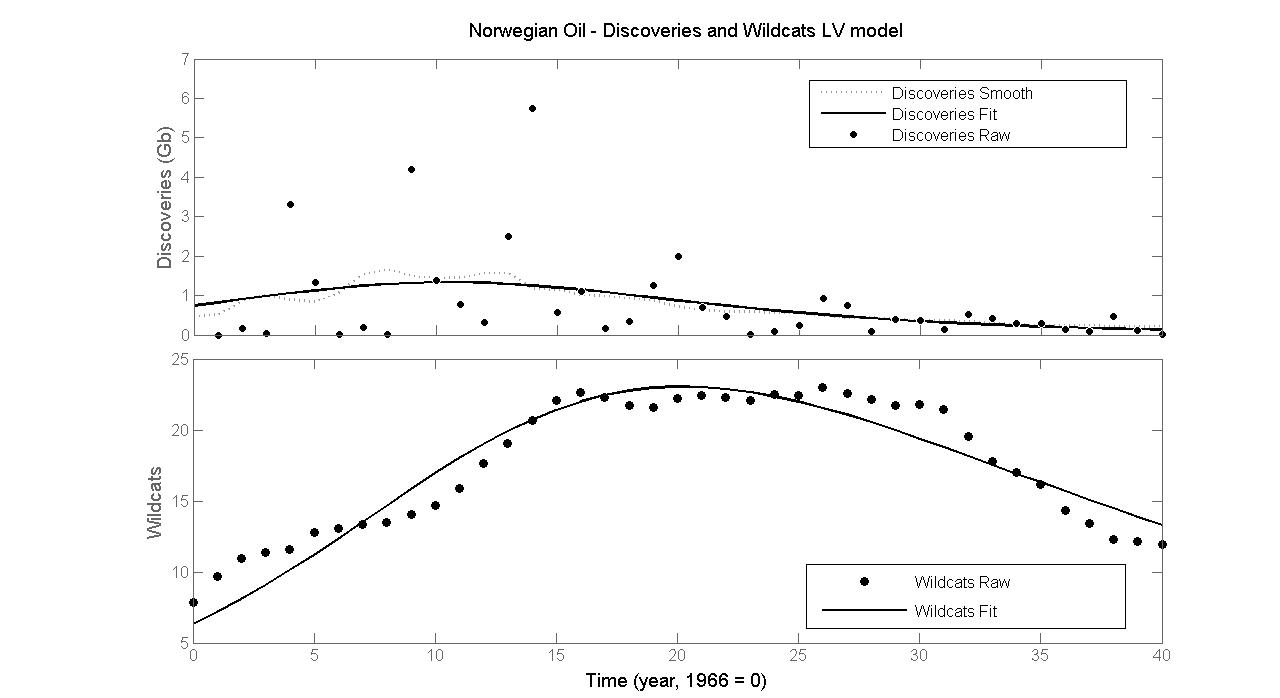
\includegraphics{fig/bardi_norwegian_oil.png}

Figure: Fitting of the data for oil discovery in Norway and of the number of wildcats. In
this case, the number of wildcats is proportional to the capital used by the oil industry in
the effort of discovering the resource, oil wells.

\href{https://www.mdpi.com/1996-1073/2/3/646}{Bardi}
\href{pdf/Bardi_2009_Hubbert_Resource_Extraction.pdf}{(pdf)}

\hypertarget{demographics}{%
\chapter{Demographics}\label{demographics}}

\hypertarget{china}{%
\section{China}\label{china}}

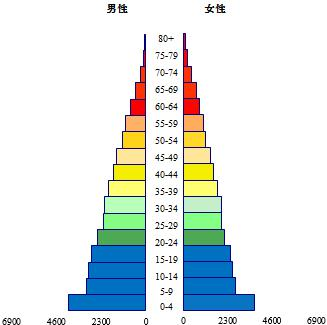
\includegraphics[width=0.3\textwidth,height=\textheight]{fig/china_demographics_1950.png}
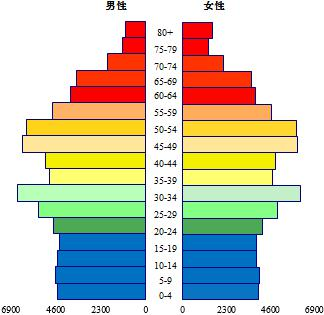
\includegraphics[width=0.3\textwidth,height=\textheight]{fig/china_demographics_2019.png}
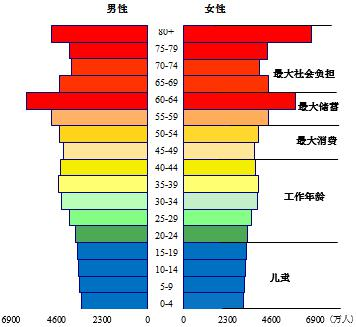
\includegraphics[width=0.3\textwidth,height=\textheight]{fig/china_demographics_2050.png}

\emph{Figure: China Population Pyramid 1950 2019 2050}

\emph{Batson}

The working paper on demographics recently published by the People's Bank of China is a pretty interesting document, and has gotten more than the usual amount of attention. It doesn't read much like the cautious, dry and technical papers previously released by this august institution. There's not much quantitative analysis or rigorous logical argument; it's more like an extended op-ed, arguing vigorously that major demographic changes for China are coming and that the country needs to wake up to that fact and adapt quickly.

This call to arms is well-timed. It seems likely that the much-delayed figures for China's 2020 population census will confirm what many demographers have been saying for a while: that China's fertility rate has been overstated, and therefore that its demographic transition and the aging of its population are going to happen even faster than standard forecasts project.

\href{https://andrewbatson.com/2021/04/28/demographics-might-change-everything-for-china-except-the-growth-model/}{Batson 2021 Demographics might change everything for China}

\emph{Hao}

Abstract: Since the industrial revolution, the death rate and birth rate have fallen successively, which has created a demographic transition and brought people to the world.
Mouth explosion, demographic dividend, aging and declining birthrate. Developed countries, as pioneers in the transition, underestimate people
The role of the population and the seriousness of aging and declining birthrates overestimate the importance of education technology, encourage childbirth, and improve the elderly.
effect. Since the founding of the People's Republic of my country, the population of our country has expanded from a rapid growth to a slowdown, and the population structure has grown from a pyramid to a long one.
It is square, and our country's population transition time is shorter, aging is faster, and declining birth rate is more serious. Our country must recognize
The demographic situation of the Qing Dynasty has changed. It is necessary to realize that the demographic dividend was used comfortably at the time, and it is a debt that needs to be repaid afterwards;
It is necessary to realize that population inertia is a huge force across generations, and its reactionary force will cause the population to change in the opposite direction;
Realize that education and technological progress cannot compensate for the decline in population. To this end, we should fully liberalize and encourage childbirth,
Really solve the difficulties of women in pregnancy, childbirth, nursery school, and school, comprehensively implement strategies, and work hard for a long time.
Now we have a long-term plan for 2035 and a century-old goal.

Memo:

\begin{enumerate}
\def\labelenumi{\arabic{enumi}.}
\tightlist
\item
  The transformation of the world population
\end{enumerate}

\begin{enumerate}
\def\labelenumi{(\arabic{enumi})}
\tightlist
\item
  The four stages of demographic transition 2
  Since the industrial revolution at the end of the eighteenth century and the beginning of the nineteenth century, 3 economic and social development has led to population deaths
  The birth rate and birth rate have successively declined, but due to the time lag between the two declines, the world has experienced ``low growth (I)
  -Accelerated Growth (II)-Growth Slowdown (III)-Low Growth (IV)'' four stages of population transformation.
  In the first stage (agricultural society before the industrial revolution is usually at this stage), productivity is underdeveloped, and the population is dead.
  The death rate is high, but in order to maintain the stability of the population size, the birth rate is usually high. This leads to the population age structure
  Pyramid shape, low dependency ratio for old age, high dependency ratio for children 4, slow economic growth.
  Phase II (initial and mid-stage of industrialization), with income growth, nutrition, hygiene and medical conditions
  Improvement, the mortality rate of the population declines rapidly, but the birth rate is usually difficult to follow. This leads to a rapid population size
  Increase, the population structure develops from a pyramid shape to a rectangular shape 5, that is, the decline in the mortality rate causes the elderly population to occupy
  The ratio and the proportion of the labor force have risen, pushing the top and middle of the pyramid to widen, but the birth rate has not decreased accordingly.
  Therefore, the bottom narrowing is not obvious. During this period, both the old-age dependency ratio and the child dependency ratio showed a downward trend.
  The growth rate is accelerating.
  In stage III (the middle and late stages of industrialization), the mortality rate of the population further decreased, but the rate of decline decreased.
  Contrary to what Malthus expected, the birth rate did not increase with the improvement of nutritional conditions, but decreased. (Google Translation)
\end{enumerate}

\href{http://www.pbc.gov.cn/redianzhuanti/118742/4122386/4122692/4214189/4215394/index.html}{Hao (2021) Cognition and countermeasures about China's population transition PBC WP2021/2}

\hypertarget{development-economics}{%
\chapter{Development Economics}\label{development-economics}}

\emph{Trainer}

Thinking about development is dominated by a conventional conception which takes
for granted the centrality of increasing production for sale, integration into the
globalized market place, moving to more sophisticated technologies, and the goal of
rising to affluent rich-world living standards. Basic criticisms of this conception of
development are briefly summarized, firstly to do with the way it has primarily
benefitted the rich and secondly regarding its grossly unsustainable resource
implications. Global biophysical resource endowments prohibit its realization. There
has been remarkably little thinking from conventional or critical sources on the goals
and means which a sustainable alternative must take. The Simpler Way project is
concerned to show the necessity for, and desirability and workability of, the
development of mostly small scale, cooperative, highly self-sufficient and self-
governing local economies focused on meeting basic needs, and not concerned with
economic growth, globalization, competing in the global market place, or aspiring to
rich-world ``living standards''. It is argued that only some form of Simpler Way can
enable satisfactory global development within sustainable resource and ecological
limits.

The major fault in most if not all previous development thinking has been
failure to grasp the need for materially simple lifestyles and systems.

Conventional development can be regarded as a form of legitimized plunder.

\textbf{Alternative, appropriate development \ldots{} The simpler way}

The basic element in appropriate development is the small, highly self-sufficient
and largely co-operative local economy.

The transition can be a process of gradually building a new ``Needs-Driven-Economy''
underneath the old ``Profit-Driven-Economy''. It can begin by a few coming together as a
Community Development Cooperative to organize the provision of some neglected basic
goods and services, for example by setting up community gardens, poultry co-ops or
aged care rosters. Their long term goal would be to increase these cooperative, socially
desirable non-market activities until they might largely replace the old economy.

\href{Trainer_2021_Third_World_Development.pdf}{Trainer (2021) Third World Development RWER 95 (pdf)}

\hypertarget{economic-measurements}{%
\chapter{Economic Measurements}\label{economic-measurements}}

\hypertarget{our-besda-economy}{%
\section{Our BESDA economy}\label{our-besda-economy}}

\hypertarget{gdp-and-ebitda}{%
\subsection{GDP and EBITDA}\label{gdp-and-ebitda}}

While the deficiencies of GDP as a measure have been well known, less emphasized has
been the fact that every single financial statement with which we build GDP exhibits the same
deficiency of being a limited barometer of value. Ironically, the main users of these financial
statements, in the business and financial sectors, are wise to the incompleteness of certain
metrics within financial statements, but act in a way that indicates they are oblivious -- or
perhaps just willing to overlook -- the incompleteness of financial statements writ large.
To explain, consider that GDP exhibits clear parallels with the profit metric of EBITDA
(earnings before interest, taxes, depreciation and amortization), Though there are technical
differences of formulation, GDP and EBITDA both represent partial measures of ``wealth
creation'' disembedded from a fuller conception of value. However, while financiers are wise
to the deficiencies of EBITDA, they have not acknowledged that the same pattern of
incompleteness reappears at the level of the overall financial statement -- and then at the yet
higher level of GDP.
With the ``DA'', EBITDA conveys the profitability of a company as if it would never again have
to spend a dollar on keeping its factories, equipment, property and software in good repair
and up to date. In other words, EBITDA excludes the cost of maintaining in good condition the
whole infrastructure upon which a company depends! It is the homeowner's fantasy of how
wealthy they would be if they never had to fix or repair anything in their house ever again.

EBITDA came to prominence during the leveraged buyout (LBO) boom of the 1980s. As
Moody's recounted in 2000: ``LBO sponsors and bankers have promoted the use of EBITDA
for its obvious image benefits. EBITDA creates the appearance of stronger interest coverage
and lower financial leverage.'' As a general rule, beware profit metrics promising image
benefits. Forbes was blunter still: ``EBITDA is essentially a tool that shows what a company

would look like if it wasn't actually that company.''
EBITDA is now clearly recognized as a ``wool-over-your-eyes'' measure, such that accounting
authorities deny it official status. It is a ``non-GAAP'' metric -- not a Generally Accepted
Accounting Principle. Its ongoing ubiquity -- besides being trivially easy to calculate -- is
because it masks the fact that a business may be overleveraged -- that it may have borrowed
against its future more than it can ever repay.

GDP is a ``wool-over-all-of-our-eyes'' metric for the same reason that it excludes the full cost
of maintaining in good condition the social and ecological infrastructure upon which the whole
economy depends. In steering society by GDP, we are effectively managing the planet on an
EBITDA basis. GDP is not just a benignly incomplete measure of wealth, it is the tool with
which we are conning ourselves.

Businesspeople -- and homeowners - know how these stories end. Eventually the under-
investment in infrastructure catches up with you. Of course, by then, you hope to have passed
the asset -- and the problem -- on to someone else. This is feasible, if not best form, where the
asset is not the whole planet. The deception works for as long as you can get away with the
under-investment and the factories and software hold up.
Buffet's partner, Charlie Munger, is characteristically more forthright on the topic:
``I think that, every time you see the phrase `EBITDA earnings', you should
substitute the phrase `bullshit earnings'.''
By analogy, GDP is ``bullshit wealth''. That we have been able to enjoy the comforts of its
deception without mishap for so long is simply because it was introduced against higher
levels of social and ecological infrastructure that we have not yet completely run down. The
under-investment is only now becoming apparent.

\hypertarget{a-besda-economy}{%
\subsection{A BESDA economy}\label{a-besda-economy}}

Long-term or ESG (environmental, social and governance) investors may protest that they
understand all this but that their own investment process insulates them from such blinkered
thinking. (``We don't use EBITDA''). Yet the point is that the whole financial system is
operating on a ``before ecological and social depreciation and amortization'' basis -- call it
BESDA, perhaps.
So, every single financial metric on the Bloomberg screen is a BESDA metric -- profits-
BESDA, earnings per share-BESDA, return on capital-BESDA, return on equity-BESDA, etc.
The millions of financial numbers processed daily by our increasingly automated markets --
which, in turn, steer our economy and drag our culture along behind, ripping up nature in its
wake -- are all BESDA numbers. It might not only be EBITDA with which we are conning
ourselves, but every financial number in the book. They all represent different degrees of
disembedded value, some of which we have unmasked, some of which we have not.
We have a sustainability challenge because the entire financial system repeats the problems
of the discredited EBITDA metric at the level of the whole economy. This is the invisible
conceptual cage we have wrapped around our decision-making and from within which the
ESG movement is frantically trying to make a difference. Alas, given the incompleteness of
our markets, the ESG movement increasingly resembles a hopeful grafting of good intentions
onto an unchallenged accounting reality that remains the largely intact source of our
problems. This is the root cause of our collective ``greenwish'' in which we are hoping that
well-intended efforts to make the world more sustainable are much closer to achieving the
necessary change than they really are

\textbf{TRUECOST}

Trucost, the sustainable consulting
firm, estimated in 2013 that large swathes of primary industry -- including agriculture and
energy companies -- would simply not be profitable if they had to pay the full costs of their
14
environmental damage. In 2011, the American Economic Review, published similar work
showing that the solid waste combustion, sewage treatment and oil- and coal-fired power
production industries generated air pollution damages -- air pollution alone -- that were greater
15
than their economic value added (EVA). On this fuller accounting perspective, these are
effectively EVS -- economic value subtracted -- industries.

\href{pdf/Austin_2021_Pigou_\%20and_the_dropped_stitch_of_economics_RWER95.pdf}{Duncan Austin: Pigou and the dropped stitch of economics RWER95 (pdf)}

\hypertarget{gdp}{%
\section{GDP}\label{gdp}}

For measurement to be accurate, the units must be stable.
Unlike natural scientists, however, economists are not in the business of
carefully defining units using universal physical constants.
Economists instead use prices, a social construct, as their unit of analysis.

The problem is that prices are unstable units of measurement.
Relative prices between commodities vary wildly over time.
This instability means that prices fail the only requirement of a good unit --- to be uniform over time.

Instead of reporting the severe uncertainty in `real' GDP, governments report a single official value.
This value hides a myriad of subjective decisions that are used to `correct' for unstable prices.

Instead of wasting time with a useless quantity that reveals nothing profound about the world,
we should seek new pluralistic methods for understanding aggregate economic activity.

Price instability translates into uncertainty in the growth of `real GDP'. While the US government reports only one official measure of `real' GDP, it quietly maintains a database of `vintage' GDP estimates. These are estimates calculated with different base years. Using this `vintage' data, we can quantify the uncertainty in the growth of `real' GDP caused by unstable prices.

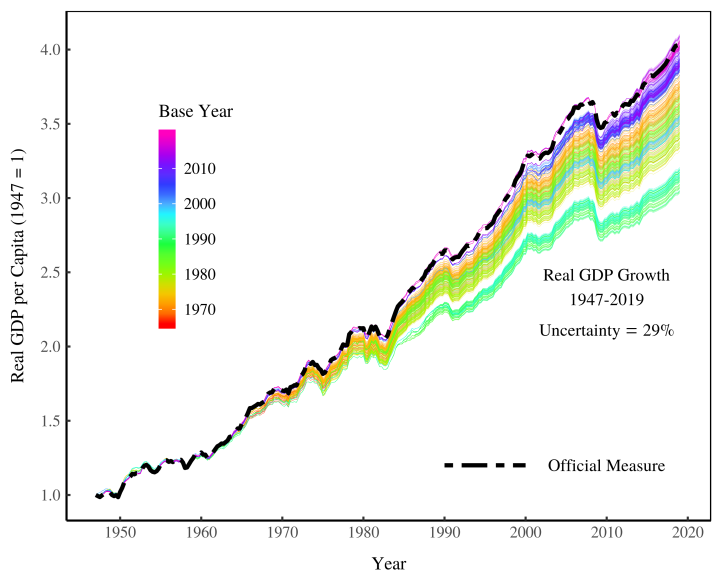
\includegraphics{fig/gdp_uncertainty_baseyear.png}

Notice that the official measure of US `real' GDP is at the upper end of the range of uncertainty. We doubt this is a coincidence. In fact, it is common for national governments to boost GDP growth by changing the base year. India recently showed a small increase in GDP growth by choosing a new base year. While this boost was small, it can sometimes be spectacularly large. Nigeria, for instance, recently changed its base year from 1990 to 2010. As a result, real GDP doubled, making Nigeria the largest economy in Africa. Base-year changes have led to similar boosts to GDP growth in Ghana, Kenya, Tanzania, Uganda and Zambia.

The NIPA Handbook, the US Bureau of Economic Analysis notes:

\begin{quote}
The fundamental problem confronting the efforts to adjust GDP and other aggregates for inflation is that there is not a single inflation number but rather a wide spectrum of goods and services with prices that are changing relative to one another over time. The index numbers for the individual components can be combined statistically to form an aggregate index, but the method of aggregation that is used affects the movements of the resulting index.
\end{quote}

\textbf{Ambigous}

The growth of `real' GDP is fundamentally uncertain. Or perhaps a better word is ambiguous.

Mainstream economists reach a very different conclusion. Their response is to simultaneously admit that calculating `real' GDP requires arbitrary choices, but then to report a single value as though it was the `truth'.

\textbf{ChainWeighting}

The US government currently calculates `real' GDP by adjusting nominal GDP with an aggregate index formed through the multiplication of successive Fisher indexes in adjacent time periods. In popular parlance, this method is called `chain-weighting'. Rather than choose a single base year in which to fix prices, chain-weighting uses a technique that resembles a rolling base year. The method is meant to simulate the effect of changing prices and spending patterns over time.
This method was adopted in the mid-1990s. The official justification was that structural changes in the US economy, especially rapidly falling computer prices, compelled the government to end the fixed base year method.

GDP treats everything with a price as contributing positively to society. Again, this comes down to the assumption that all prices reveal utility. If machine guns sell for the same price as MRI machines, neoclassical theory tells us that both contribute the same utility to society.

In response to such absurdities, ecological economists have developed alternative indicators that subtract the value of social `bads' from the value of social `goods'. While well-motivated, this approach still assumes that we can aggregate the `real' value of `goods' and `bads'. But because prices are unstable, this aggregate is still ill-defined.

`Real' GDP is a regressive measure of social progress. Not only is it ill-defined and based on flawed premises, it equates market value with social welfare. This justifies the income of the powerful.

\textbf{Alternatives}

The key, we believe, is to separate the study of economic distribution from the study of economic scale. The former is the appropriate domain of prices. The latter is best measured using biophysical units.

\emph{Prices: Distribution}

We believe it is important to distinguish between economic \emph{distribution} and economic \emph{scale}.
`Real' GDP assumes that prices can be used to measure economic scale.
In contrast, we assume that prices do nothing of the sort.
Prices are a tool for distributing resources.
The proper place for prices, then, is for understanding economic distribution.

\emph{Scale: Energy}

To measure the scale of the economy, we think it is appropriate to focus on energy. Physicist Eric Chaisson argues that energy is the universal currency of science. By measuring economic scale using energy, we put economics in line with the rest of science. And if we are concerned with sustainability, there is no better starting point than to focus on energy use. After all, the profligate use of fossil fuels under a capitalist economy is the primary driver of climate change.

Energy has many forms as it is flows through society. One possibility is to focus on primary energy consumption, and see how this relates to changes in social structure. Another possibility is to measure `useful work' --- the consumption of end-use energy. Still another possibility is to measure the aggregate flow rate, which is a measure of all annual energy conversions in an economic system.

The study of economic growth, which should focus on biophysical flows.

Continuing to use `real' GDP as a measure of social progress implicitly accepts a theory
(neoclassical economics) that has long been used as an ideological justification for capitalist power.

\href{https://economicsfromthetopdown.com/2019/12/15/why-we-should-abandon-real-gdp-as-a-measure-of-economic-activity/}{Fix GDP}

\hypertarget{economic-modelling}{%
\chapter{Economic Modelling}\label{economic-modelling}}

\emph{Bookstaber}

The End of Theory: Financial Crises, the Failure of Economics, and the Sweep of Human Interaction

Our economy may have recovered from the Great Recession---but not our economics. In The End of Theory, Richard Bookstaber discusses why the human condition and the radical uncertainty of our world renders the standard economic model---and the theory behind it---useless for dealing with financial crises. What model should replace it? None. At least not any version we've been using for the past two hundred years. Instead, Bookstaber argues for a new approach called agent-based economics, one that takes as a starting point the fact that we are humans, not the optimizing automatons that standard economics assumes we are.

Bookstaber's groundbreaking paradigm promises to do a far better job at preventing crises and managing those that break out. As he explains, our varied memories and imaginations color our economic behavior in unexpected hues. Agent-based modeling embraces these nuances by avoiding the mechanistic, unrealistic structure of our current economic approach. Bookstaber tackles issues such as radical uncertainty, when circumstances take place beyond our anticipation, and emergence, when innocent, everyday interactions combine to create sudden chaos. Starting with the realization that future crises cannot be predicted by the past, he proposes an approach that recognizes the human narrative while addressing market realities.

Sweeping aside the historic failure of twentieth-century economics, The End of Theory offers a novel and innovative perspective, along with a more realistic and human framework, to help prevent today's financial system from blowing up again.

\href{https://press.princeton.edu/books/hardcover/9780691169019/the-end-of-theory}{Bookstaber (Book Page)}

\hypertarget{tax}{%
\chapter{Tax}\label{tax}}

\hypertarget{corporate-tax}{%
\section{Corporate Tax}\label{corporate-tax}}

\textbf{Profit Shifting}

\emph{OECD Process}

There remain significant difficulties in the OECD process, with its two-pillar proposals. First, there is no common ground on `Pillar One'. This is the element which would go beyond the archaic arm's length principle and introduce some element of formulary apportionment (that is, allocating a share of each multinational's global profits to the places where they actually do business, in the form of sales and employment). The US (under Biden, as under Trump) wants Pillar One to apply to all businesses; the EU is focused on the big tech multinationals; and the OECD proposal to identify `consumer-facing' businesses falls somewhere in between these.

As things stand, the OECD proposal is highly complex and would retain arm's length pricing for most profits, and therefore result in relatively little reduction in profit shifting -- making it largely unattractive for most countries. At the same time, the proposal would require global treaty change, meaning that it could very easily be blocked -- including by the US Congress, regardless of whether the Biden administration had come around to support it.

`Pillar Two' contemplates a global minimum corporate tax rate. This has the potential to go a long way to stop profit shifting, not by making it harder to achieve but by making it much less rewarding -- since multinationals would, in theory, end up being taxed at the minimum rate even if they managed to shift the profits to a zero rate jurisdiction.

Here again though, the current OECD proposals are highly complex, and have been very unambitious. And an argument about `rule order' -- in simple terms, whether the home country of a multinational goes first in levying any top-up tax, or the various host countries -- has exposed the major distributional question. Despite some initial optimism, most non-OECD members have by now become thoroughly disillusioned with the process. An outcome that favours OECD members, despite lower-income countries bearing disproportionately high revenue losses due to profit shifting, would be unconscionable -- but, sadly, not entirely unexpected.

Lastly, the insistence that the two pillars are inseparable, and must be delivered jointly, creates a hugely complicated contraption requiring great resources to move ahead, but with little certainty over any benefits.

\emph{Way Forward}

Stepping out of the limitations of the OECD process, things very quickly start to look much brighter. This is for three main reasons.

First, the two pillars can be separated -- and that means the unworkable and unambitious `Pillar One' can be left behind, along with the requirement for global treaty change. Instead, a global minimum corporate tax can be taken forward by a coalition of the willing. (In fairness to the OECD secretariat, they have raised this possibility at times also, recognising the practical difficulties of their Pillar One.) With the US and Germany (and the European Commission) committed to a minimum tax, broad agreement on the shape could be reached relatively quickly.

Second, the OECD leadership's longstanding insistence on a very low minimum rate of 12.5\% can be set aside. The Biden administration has indicated a rate of 21\%. The Independent Commission for the Reform of International Corporate Taxation has proposed 25\% as an absolute minimum; while discussions among various groups of lower-income countries have suggested higher rates still, to ensure that they are not disadvantaged. Negotiating upwards from 21\% -- and with the possibility of different countries taking their own approaches as appropriate -- would provide a quite different dynamic.

And third, the setting aside of Pillar One creates the possibility of pursuing a more ambitious approach to the minimum tax. Our proposal for the METR, or Minimum Effective Tax Rate for multinationals, does just this. We propose a method that builds on the technical efforts of the OECD secretariat, who have done sterling work in establishing various approaches to identify and to apportion taxable profits, but shifts the politics substantially.

\emph{METR}

In effect, the METR combines the two pillars by identifying under-taxed profits, and then apportioning these for `top-up' taxation on a formulary basis, according to the location of multinationals' real activity. In this way, the METR cuts through any `rule order' debates and instead treats all countries, home or host, on an equivalent basis.

Politically, the momentum for globally inclusive solutions at the UN, rather than the rich countries' club at the OECD, will continue to grow -- and especially if a one-sided minimum tax solution emerges from the OECD now. The FACTI panel report called for the negotiation of a UN tax convention, which would provide the basis for an intergovernmental body under UN auspices to set corporate tax rules in future -- including a global minimum tax rate designed to benefit all.

That the US administration is now leading the push for an ambitious global minimum tax rate confirms this as the new norm. The decisions set to be made in the next couple of months, over technical design and political inclusion, will determine just how effective this can be in bringing an end -- finally -- to the decades-long race to the bottom in corporate tax.

With the confirmation of this new narrative, it seems likely that what is left undone in the OECD process will be resolved through a combination of unilateral and UN action.

\href{https://www.taxjustice.net/2021/04/07/us-treasury-secretary-yellen-confirms-its-time-to-end-the-race-to-the-bottom-on-corporate-tax/}{Global Corporate Minimum Tax}

\hypertarget{economists}{%
\chapter{Economists}\label{economists}}

\hypertarget{joan-robinson}{%
\section{Joan Robinson}\label{joan-robinson}}

In the autumn of 1975, there was one name ``on everyone's list for this year's Nobel Prize in Economics,'' Business Week magazine trumpeted: the Cambridge economist Joan Robinson. The week before the prize announcement, the magazine predicted that Robinson would be the first woman to win the prize. A major interpreter of John Maynard Keynes and Karl Marx, she was one of the most prominent economists of her generation.

But when the names of the winners were read out at the Royal Swedish Academy of Sciences, Robinson's name was not among them. When she died in 1983, just shy of her eightieth birthday, she had not won the prize -- despite words of support from laureates as different as Paul Samuelson and Milton Friedman.

What went wrong? More than perhaps any other factor, one man was to blame: Mao Zedong. Robinson's writing in praise of Mao's China -- from her defense of the ruinous Great Leap Forward to her zesty praise of the Cultural Revolution -- was likely what lost her the Prize. Fang Qin, an economist at Fudan University in Shanghai, put it plainly: ``She is considered the most important female economist in history, but she did not win the Nobel Prize because she publicly praised the Cultural Revolution.''

``How could it happen that, under cover of Mao Tse-tung thought, a medieval drama of ambition and treachery could play itself out?''

\href{https://chinachannel.org/2017/12/13/fellow-travellers-tale/}{Gewirtz (2017) Mao NobelPrize}

\hypertarget{part-appendices}{%
\part{Appendices}\label{part-appendices}}

\hypertarget{appendix-appendices}{%
\appendix}


\hypertarget{about}{%
\chapter{About}\label{about}}


\includegraphics{fig/me.jpg}

\emph{Dyre Haugen} and \emph{Dyrehaugen} is Webian for \emph{Jon Martin} -
self-owned Globian, Webian, Norwegian and Canarian with
a background from industrial research policy, urban planning and
economic development consulting on global, regional and urban scales.
I am deeply concerned about the (insane) way
humanity (i.e.~capitalism) interfere with nature.
In an effort to gain insights in how and why this happens
stuff is collected from around the web and put together
in a linked set of web-sites.
The sites are operated as personal notebooks.
However, these days things can be easily published to the
benefit of others concerned with the same issues.
But be aware - this is not polished for presentation or
peer-reviewed for exactness.
I offer you just to have a look at my `work-desk' as it appears in the moment.
Any comment or suggestion can be mailed to \href{mailto:dyrehaugen@gmail.com}{\nolinkurl{dyrehaugen@gmail.com}}
You can follow me on twitter as @dyrehaugen.
Thanks for visiting!

\hypertarget{links}{%
\chapter{Links}\label{links}}

\textbf{Current Dyrehaugen Sites:}

\begin{itemize}
\tightlist
\item
  \href{https://dyrehaugen.github.io/rcap}{rcap - On Capitalism} \href{http://localhost/rcap}{(loc)}
\item
  \href{https://dyrehaugen.github.io/rclm}{rclm - On Climate Change} \href{http://localhost/rclm}{(loc)}
\item
  \href{https://dyrehaugen.github.io/recs}{recs - On Economics} \href{http://localhost/recs}{(loc)}
\item
  \href{https://dyrehaugen.github.io/rngy}{rfin - On Finance} \href{http://localhost/rfin}{(loc)}
\item
  \href{https://dyrehaugen.github.io/rngy}{rngy - On Energy} \href{http://localhost/rngy}{(loc)}
\item
  \href{https://dyrehaugen.github.io/renv}{renv - On Environment} \href{http://localhost/renv}{(loc)}
\item
  \href{https://dyrehaugen.github.io/rsts}{rsts - On Statistics} \href{http://localhost/rsts}{(loc)}
\item
  \href{https://dyrehaugen.github.io/rurb}{rurb - On Urbanization} \href{http://localhost/rurb}{(loc)}
\item
  \href{https://dyrehaugen.github.io/rvar}{rvar - On Varia} \href{http://localhost/rvar}{(loc)}
\item
  \href{https://dyrehaugen.github.io/rwsd}{rwsd - On Wisdom} \href{http://localhost/rwsd}{(loc)}
\end{itemize}

\textbf{Blogs:}

\begin{itemize}
\tightlist
\item
  \href{https://dyrehaugen.github.io/rde}{rde - Blog in English} \href{http://localhost/rde}{(loc)}
\item
  \href{https://dyrehaugen.github.io/rdn}{rdn - Blog in Norwegian} \href{http://localhost/rdn}{(loc)}
\end{itemize}

\textbf{Discontinued:}

\begin{itemize}
\tightlist
\item
  \href{https://dyrehaugen.github.io/jdt}{jdt - Collection (Jekyll)} \href{http://localhost/jdt}{(loc)}
\item
  \href{https://dyrehaugen.github.io/hdt}{hdt - Collection (Hugo)} \href{http://localhost/hdt}{(loc)}
\end{itemize}

\textbf{Not listed:}

\begin{itemize}
\tightlist
\item
  (q:) dhe dhn jrw56
\item
  (z:) rcsa rpad rstart
\end{itemize}

\hypertarget{news}{%
\chapter{NEWS}\label{news}}

  \bibliography{book.bib,packages.bib}

\end{document}
